\documentclass[10pt,a4paper]{article}

% ---------------------------------------------------------------------------
% Pacotes
% ---------------------------------------------------------------------------
\usepackage[a4paper,margin=2cm]{geometry}
\usepackage[T1]{fontenc}
\usepackage[utf8]{inputenc}
\usepackage{lmodern}
\usepackage{babel}
\babelprovide[import, main]{brazilian}
\usepackage{microtype}
\usepackage{amsmath,amssymb}
\usepackage{graphicx}
\usepackage{booktabs}
\usepackage{array}
\usepackage{tabularx}
\usepackage{multirow}
\usepackage{makecell}
\usepackage[font=small,labelfont=bf,skip=4pt]{caption}
\usepackage{enumitem}
\usepackage{xcolor}
\usepackage{tikz}
\usetikzlibrary{arrows.meta}
\usepackage[hidelinks]{hyperref}
\hypersetup{pdftitle={Busca Híbrida, Reranking e RAG no NFCorpus},
            pdfauthor={Leonardo D. Demore; Arthur Araujo}}

% As figuras ficam em trabalho2/results/ (compilando a partir da raiz do
% repositório); os demais caminhos permitem compilar de outros diretórios.
\graphicspath{{trabalho2/results/}{results/}{./}}

\setlist[itemize]{leftmargin=1.1em, itemsep=1pt, parsep=0pt, topsep=2pt}
\setlist[enumerate]{leftmargin=1.5em, itemsep=1pt, parsep=0pt, topsep=2pt}
\setlength{\emergencystretch}{3em}
\renewcommand{\topfraction}{0.9}
\renewcommand{\bottomfraction}{0.8}
\renewcommand{\textfraction}{0.1}
\renewcommand{\floatpagefraction}{0.8}
\setlength{\textfloatsep}{12pt plus 2pt minus 2pt}
\setlength{\intextsep}{10pt plus 2pt minus 2pt}

% ---------------------------------------------------------------------------
% Macros
% ---------------------------------------------------------------------------
\newcommand{\med}[1]{\mbox{MED-#1}}         % documento do NFCorpus
\newcommand{\pq}[1]{\mbox{PLAIN-#1}}        % consulta do NFCorpus
\newcommand{\ri}[1]{\textbf{#1}}            % relevante de grau 1 (tabelas)
\newcommand{\rii}[1]{\textbf{#1}\textsuperscript{2}} % relevante de grau 2
\newcommand{\sep}{\ \textperiodcentered\ }
\newcommand{\gn}{\ensuremath{-}}            % sinal de menos em texto

\begin{document}

% ---------------------------------------------------------------------------
% Cabeçalho
% ---------------------------------------------------------------------------
\begin{center}
{\LARGE\bfseries Busca Híbrida, Reranking e RAG no NFCorpus\par}
\vspace{3pt}
{\large SCC0282 -- Recuperação de Informação -- Trabalho Prático 2\par}
\vspace{12pt}
{\large Leonardo D. Demore (15674786) \qquad Arthur Araujo (14651458)\par}
\vspace{4pt}
{\small Instituto de Ciências Matemáticas e de Computação (ICMC) -- Universidade de São Paulo (USP), São Carlos\par}
\vspace{2pt}
{\small\texttt{leodemore@usp.br}, \texttt{arthurhsilvaaraujo@usp.br}\par}
\end{center}

% ===========================================================================
\section{Introdução}
% ===========================================================================

Sistemas de Recuperação de Informação (RI) modernos raramente dependem de um único modelo. Um modelo lexical como o BM25 pontua documentos pela sobreposição ponderada de termos com a consulta: é rápido, interpretável e preciso quando a consulta contém termos raros que aparecem literalmente nos relevantes, mas atribui score zero a qualquer documento que trate do assunto com outras palavras. Esse foi o limite apontado no Trabalho~1. Modelos densos (\emph{bi-encoders}) representam consultas e documentos como vetores num espaço semântico e lidam com paráfrase e variação de vocabulário, ao custo de diluir termos específicos. Sistemas atuais combinam os dois, refinam o topo do ranking com modelos mais caros (\emph{cross-encoders}) e usam os documentos recuperados como evidência para que uma LLM gere respostas (\emph{Retrieval-Augmented Generation}, RAG). Entender como esses componentes interagem exige mais do que médias: é preciso examinar consultas concretas e localizar em que estágio cada acerto ou erro acontece.

O objetivo deste trabalho é implementar e avaliar esse pipeline completo sobre o \textbf{NFCorpus} (versão do BEIR), uma coleção biomédica de consultas curtas: (i)~busca lexical com \textbf{BM25} sobre um índice invertido implementado do zero; (ii)~\textbf{correção ortográfica} de termos desconhecidos com k-gramas, coeficiente de Jaccard e distância de edição; (iii)~\textbf{busca semântica} com um bi-encoder pré-treinado; (iv)~\textbf{busca híbrida} por \emph{Reciprocal Rank Fusion} (RRF); (v)~\textbf{reranking} com cross-encoder; e (vi)~\textbf{RAG} com uma LLM local, comparado a respostas sem RAG por avaliação humana às cegas. Todas as escolhas de modelos e parâmetros foram feitas no conjunto dev, e o test foi usado só na avaliação final. O índice invertido, o BM25, o corretor ortográfico, o RRF e todas as métricas foram implementados pelo grupo em Python; bibliotecas foram usadas para stopwords, stemming e lematização (nltk), embeddings e cross-encoders (sentence-transformers), execução da LLM (Ollama), conferência das métricas (ir\_measures), concordância entre avaliadores (scikit-learn) e tabelas e gráficos (pandas, matplotlib).

% ===========================================================================
\section{Metodologia}
% ===========================================================================

A Figura~\ref{fig:pipeline} resume o pipeline e os componentes escolhidos. Esta seção descreve cada etapa e as decisões tomadas; as escolhas feitas no dev aparecem junto da etapa correspondente, e o protocolo de avaliação está na Seção~\ref{sec:avaliacao}.

\begin{figure}[!htb]
\centering
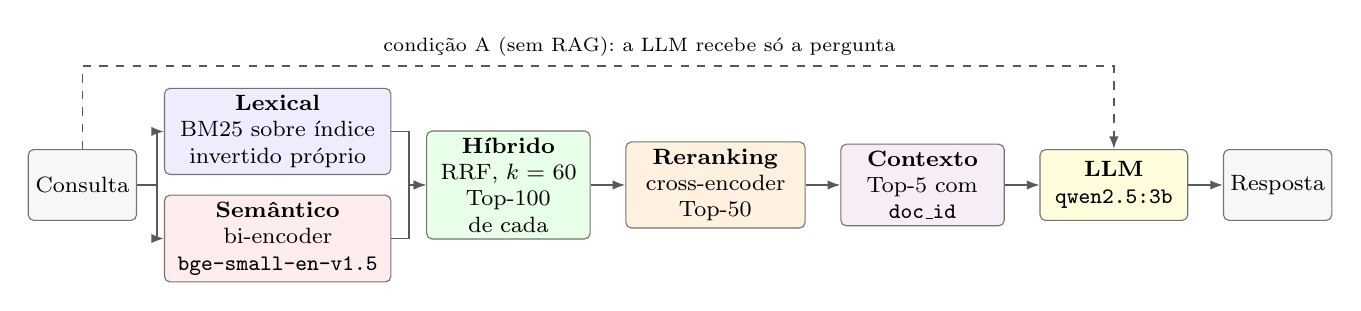
\begin{tikzpicture}[
  font=\footnotesize, >={Latex[length=1.6mm]},
  box/.style={draw=black!55, rounded corners=2pt, align=center, inner sep=2.5pt,
              minimum height=9mm, fill=black!3},
  arr/.style={->, draw=black!65, semithick}]
  \node[box, text width=1.2cm] (q) at (0.69,0) {Consulta};
  \node[box, fill=blue!7, text width=2.7cm] (lex) at (3.17,0.68) {\textbf{Lexical}\\BM25 sobre índice\\invertido próprio};
  \node[box, fill=red!7, text width=2.7cm] (sem) at (3.17,-0.68) {\textbf{Semântico}\\bi-encoder\\\texttt{bge-small-en-v1.5}};
  \node[box, fill=green!9, text width=1.9cm] (rrf) at (6.10,0) {\textbf{Híbrido}\\RRF, $k=60$\\Top-100 de cada};
  \node[box, fill=orange!12, text width=2.1cm] (ce) at (8.73,0) {\textbf{Reranking}\\cross-encoder\\Top-50};
  \node[box, fill=violet!7, text width=1.9cm] (ctx) at (11.36,0) {\textbf{Contexto}\\Top-5 com\\\texttt{doc\_id}};
  \node[box, fill=yellow!14, text width=1.7cm] (llm) at (13.79,0) {\textbf{LLM}\\\texttt{qwen2.5:3b}};
  \node[box, text width=1.2cm] (ans) at (15.87,0) {Resposta};
  \draw[arr] (q.east) -- ++(0.25,0) |- (lex.west);
  \draw[arr] (q.east) -- ++(0.25,0) |- (sem.west);
  \draw[arr] (lex.east) -- ++(0.22,0) |- (rrf.west);
  \draw[arr] (sem.east) -- ++(0.22,0) |- (rrf.west);
  \draw[arr] (rrf) -- (ce);
  \draw[arr] (ce) -- (ctx);
  \draw[arr] (ctx) -- (llm);
  \draw[arr] (llm) -- (ans);
  \draw[arr, dashed] (q.north) -- ++(0,1.05) -| node[pos=0.27, above, font=\scriptsize]{condição A (sem RAG): a LLM recebe só a pergunta} (llm.north);
\end{tikzpicture}
\caption{Pipeline do sistema com os componentes escolhidos no dev. O índice invertido e os embeddings dos documentos são calculados uma única vez. No experimento de RAG, a condição B (com RAG) percorre o pipeline inteiro, e a condição A (tracejado) envia só a pergunta à mesma LLM. A correção ortográfica é um experimento separado (Seção~\ref{sec:met-erros}); os demais experimentos usam as consultas originais.}
\label{fig:pipeline}
\end{figure}

% ---------------------------------------------------------------------------
\subsection{Pré-processamento}
% ---------------------------------------------------------------------------

Cada documento é representado pela concatenação de \texttt{title} e \texttt{text}, com um ponto entre os dois quando o título não termina em pontuação, e a \emph{mesma} string é usada nos três sistemas (lexical, semântico e reranking). A normalização converte o texto para minúsculas e remove acentos e símbolos não ASCII por decomposição Unicode NFKD ($\beta$-carotene $\to$ \texttt{carotene}, Ménière $\to$ \texttt{meniere}); a tokenização usa a expressão regular \texttt{[a-z0-9]+}, como no Trabalho~1. Os dígitos são mantidos porque carregam sentido no domínio (\emph{omega~3}, \emph{b12}, \emph{type 2 diabetes}). A remoção de stopwords (lista do NLTK para inglês, 198 palavras) é feita \emph{antes} da redução morfológica: na ordem inversa, o Porter transformaria \emph{does} em \texttt{doe}, que escaparia da lista. Consultas e documentos passam pelo mesmo pipeline. Comparamos cinco configurações com o BM25 nos valores usuais ($k_1 = 1{,}2$, $b = 0{,}75$) e escolhemos a de maior NDCG@10 médio no dev (Tabela~\ref{tab:preproc}).

\begin{table}[!htb]
\centering\small
\caption{Configurações de pré-processamento: efeito sobre a coleção e desempenho do BM25 ($k_1 = 1{,}2$, $b = 0{,}75$) nas 324 consultas do dev. Em negrito, a configuração escolhida.}
\label{tab:preproc}
\begin{tabular}{@{}lrrrcc@{}}
\toprule
Configuração & Vocabulário & Termos (total) & Termos/doc & NDCG@10 (dev) & MAP@10 (dev) \\
\midrule
\textbf{\texttt{stopwords+stemming}} & 19.398 & 600.433 & 165,3 & \textbf{0,2957} & \textbf{0,0922} \\
\texttt{stemming}                    & 19.496 & 890.831 & 245,2 & 0,2897 & 0,0891 \\
\texttt{stopwords+lematização}       & 24.388 & 600.433 & 165,3 & 0,2884 & 0,0867 \\
\texttt{stopwords}                   & 26.740 & 600.433 & 165,3 & 0,2747 & 0,0806 \\
\texttt{nada}                        & 26.869 & 890.831 & 245,2 & 0,2678 & 0,0791 \\
\bottomrule
\end{tabular}
\end{table}

\begin{itemize}
\item \textbf{Escolhida: \texttt{stopwords+stemming}}, a mesma do Trabalho~1. A ordem das quatro configurações comuns aos dois trabalhos se repete (\texttt{nada} $<$ \texttt{stopwords} $<$ \texttt{stemming} $<$ \texttt{stopwords+stemming}), mesmo com outra coleção, outro domínio e consultas bem mais curtas, e NDCG@10 e MAP@10 concordam na ordenação das cinco.
\item \textbf{As duas etapas agem em eixos diferentes.} Remover stopwords corta 32,6\% dos tokens (890.831 $\to$ 600.433), mas só 129 termos do vocabulário: o ganho é sobretudo de eficiência, e o de efetividade é pequeno (+2,6\% de NDCG@10 sobre \texttt{nada}). O stemming não muda o total de tokens e corta 27,4\% do vocabulário; é dele o maior ganho (+8,2\% sozinho e +10,4\% combinado com stopwords).
\item \textbf{Lematização $\times$ stemming.} A lematização do WordNet, sem etiquetagem gramatical (todo termo tratado como substantivo), é muito mais conservadora: reduz o vocabulário em 8,8\% contra 27,5\% do Porter sobre a mesma base, e só 2.345 formas agrupam mais de um termo, contra 4.154. Ela une flexões de número (\emph{studies} $\to$ \texttt{study}, \emph{women} $\to$ \texttt{woman}); o Porter também une derivações (\emph{infected}, \emph{infections} $\to$ \texttt{infect}) e famílias inteiras (\emph{activate}, \emph{activation}, \emph{active} $\to$ \texttt{activ}). No dev, a lematização entrega 65\% do ganho do stemming sobre a base \texttt{stopwords} (+0,0137 contra +0,0210). A agressividade do Porter tem custo visível (\emph{organ}, \emph{organic}, \emph{organism} e \emph{organization} viram \texttt{organ}), mas no agregado casar mais variantes compensa.
\end{itemize}

% ---------------------------------------------------------------------------
\subsection{Índice invertido}
% ---------------------------------------------------------------------------

O índice foi implementado do zero com estruturas genéricas do Python (\texttt{dict}, \texttt{list} e \texttt{Counter}). O \textbf{dicionário} é um \texttt{dict} termo $\to$ posting list, com acesso O(1). Cada \textbf{posting list} é uma lista de pares \texttt{(doc\_idx, tf)} em ordem crescente de \texttt{doc\_idx}, ordem que sai naturalmente da construção sequencial; o \texttt{doc\_idx} (posição do documento na coleção) ocupa menos memória que a string \texttt{MED-xxxx}. O índice guarda ainda o comprimento de cada documento, $N$ e o comprimento médio (avgdl); o df é o tamanho da posting list. É tudo o que o BM25 precisa, e o índice não depende de $k_1$ e $b$. A busca é \textbf{term-at-a-time}: para cada termo da consulta percorre-se só a sua posting list, acumulando os scores num dicionário de acumuladores, de modo que documentos sem nenhum termo da consulta nunca são visitados. Como verificação, df e tf de quatro termos (\emph{statin}, \emph{cancer}, \emph{vitamin}, \emph{broccoli}) batem com uma contagem direta sobre os documentos, e todas as posting lists estão ordenadas e sem duplicatas. A Tabela~\ref{tab:indice} traz as estatísticas do índice da configuração escolhida.

\begin{table}[!htb]
\centering\small
\caption{Índice invertido (\texttt{stopwords+stemming}). Tempos medidos em CPU; o tempo por consulta inclui o pré-processamento da consulta, o acúmulo dos scores e a ordenação, nas 323 consultas de test.}
\label{tab:indice}
\begin{tabular}{@{}ll@{}}
\toprule
Medida & Valor \\
\midrule
Termos no vocabulário & 19.398 (9.041 com df $=1$, 47\%) \\
Postings (total) & 359.738 (média de 18,5 por termo; mediana 2) \\
Comprimento médio do documento (avgdl) & 165,3 termos \\
Construção do índice & 0,21 s (média de 5; pré-processamento da coleção: 0,35 s) \\
Tempo médio por consulta & 0,44 ms \\
Documentos visitados por consulta & 494,2 em média (13,6\% da coleção); máximo de 2.803 \\
\bottomrule
\end{tabular}
\end{table}

A distribuição das postings é muito assimétrica: a média é de 18,5 por termo, mas a mediana é 2. Os termos genéricos do domínio têm milhares de postings e dominam o custo: o pior caso, \pq{1262} (\emph{Global Burden of Disease Study}), visita 2.803 documentos (77\%) porque \texttt{studi} aparece em 2.364 documentos e \texttt{diseas} em 1.149. Mesmo assim, só as posting lists dos termos da consulta são lidas.

% ---------------------------------------------------------------------------
\subsection{Busca lexical (BM25)}
% ---------------------------------------------------------------------------

Escolhemos o \textbf{BM25} como baseline lexical. No Trabalho~1 ele superou o Modelo Vetorial nas quatro métricas e nas quatro configurações de pré-processamento (+12,2\% de MAP na Cranfield), e a explicação encontrada foi a normalização parcial e ajustável pelo comprimento ($b$) somada à saturação da tf ($k_1$), enquanto o cosseno penaliza documentos longos pela norma completa do vetor. No NFCorpus os documentos vão de poucas dezenas a cerca de 1.500 palavras, o que torna essa diferença relevante. A função de score é a do Trabalho~1, adaptada ao novo índice:
\[
\mathrm{BM25}(q,d) = \sum_{t \in q} \mathrm{qtf}_t \cdot \mathrm{idf}_t \cdot
\frac{\mathrm{tf}_{t,d}\,(k_1+1)}{\mathrm{tf}_{t,d} + k_1\bigl(1 - b + b\,\frac{|d|}{\mathrm{avgdl}}\bigr)},
\qquad
\mathrm{idf}_t = \ln\Bigl(1 + \frac{N - \mathrm{df}_t + 0{,}5}{\mathrm{df}_t + 0{,}5}\Bigr).
\]
O deslocamento $1+\cdots$ no idf evita valores negativos para termos presentes em mais da metade dos documentos. O ranking contém todos os documentos com score não nulo, em ordem decrescente, com desempate pelo \texttt{doc\_idx} para ser reprodutível. Com o pré-processamento fixado, variamos $k_1$ e $b$ num grid $5 \times 5$ no dev; como $k_1$ e $b$ são parâmetros de busca, o índice não é reconstruído (Tabela~\ref{tab:grid}).

\begin{table}[!htb]
\centering\small
\caption{Grid de parâmetros do BM25: NDCG@10 médio no dev. Em negrito, o melhor ponto; em itálico, os valores usuais.}
\label{tab:grid}
\begin{tabular}{@{}c ccccc@{}}
\toprule
$k_1 \backslash b$ & 0,3 & 0,5 & 0,75 & 0,9 & 1,0 \\
\midrule
0,6 & 0,2912 & 0,2932 & 0,2926 & 0,2921 & 0,2898 \\
0,9 & 0,2929 & 0,2948 & 0,2946 & 0,2941 & 0,2921 \\
1,2 & 0,2947 & 0,2962 & \emph{0,2957} & 0,2965 & 0,2938 \\
1,5 & 0,2954 & 0,2969 & 0,2963 & 0,2959 & 0,2933 \\
2,0 & 0,2945 & \textbf{0,2977} & 0,2956 & 0,2952 & 0,2939 \\
\bottomrule
\end{tabular}
\end{table}

\begin{itemize}
\item \textbf{O grid é plano.} Nas 25 combinações o NDCG@10 vai só de 0,2898 a 0,2977 (2,7\%), e o melhor ponto ($k_1 = 2{,}0$, $b = 0{,}5$) supera os valores usuais em apenas \textbf{0,7\%}. Pelo protocolo adotamos o melhor ponto do dev, mas uma diferença desse tamanho não deve ser lida como ganho robusto: é a mesma conclusão do Trabalho~1, em que o melhor ponto rendia +1,8\%.
\item \textbf{$b = 1$ (normalização total) é o pior valor em todas as linhas}, e $b$ entre 0,5 e 0,9 é praticamente indiferente; $k_1$ maior (saturação mais lenta da tf) ajuda um pouco até 1,5--2,0.
\item \textbf{O comprimento não explica a preferência por $b$ menor.} Os 3.119 documentos julgados relevantes no dev têm comprimento médio de 165,1 termos, igual ao avgdl da coleção (165,3). Diferente do Trabalho~1, em que os relevantes longos separavam os modelos, aqui não há viés de comprimento nos julgamentos, o que é coerente com a planura do grid.
\end{itemize}

% ---------------------------------------------------------------------------
\subsection{Tolerância a erros}
\label{sec:met-erros}
% ---------------------------------------------------------------------------

O \textbf{dicionário} é formado pelos 26.869 termos da coleção \emph{antes} do stemming (a saída da tokenização sobre todos os documentos, com stopwords), com a frequência de cada um na coleção (cf). Os termos da consulta passam pela mesma normalização. A correção segue o pipeline de Manning et al.\ (2008, cap.~3):
\begin{enumerate}
\item \textbf{Detecção.} Um termo é desconhecido se não está no dicionário; números nunca são corrigidos. Um termo fora do dicionário cujo radical de Porter \emph{já existe no índice lexical} também não é corrigido (\emph{proteção de variantes morfológicas}), porque já casa com o índice após o stemming; é o caso de \emph{deafness}, \emph{pineapples} e \emph{cataracts} em consultas de test.
\item \textbf{Geração de candidatos por k-gramas.} O termo recebe marcadores de fronteira (\texttt{\$termo\$}) e é quebrado em k-gramas; um índice invertido de k-gramas (k-grama $\to$ termos do dicionário) devolve todos os termos que compartilham ao menos um k-grama com ele.
\item \textbf{Filtro por Jaccard.} $J(A,B) = |A \cap B|/|A \cup B|$ entre os conjuntos de k-gramas; candidatos com $J < \tau$ são descartados.
\item \textbf{Seleção por distância de edição.} Entre os que passam, vence o de menor distância de \textbf{Damerau-Levenshtein restrita} (\emph{optimal string alignment}), em que a troca de dois caracteres adjacentes custa 1, e não 2 como na Levenshtein, porque a transposição é um dos quatro tipos de erro do experimento. Desempate: maior Jaccard e, depois, maior cf. Se nenhum candidato estiver a no máximo 2 edições, o termo fica como está.
\end{enumerate}

\textbf{Ajuste no dev.} Escolhemos $k \in \{2, 3\}$ e $\tau \in \{0{,}1; \dots; 0{,}5\}$ pela acurácia (fração de casos em que o termo corrigido é exatamente o original) sobre \textbf{2.079 erros sintéticos}: para cada um dos 521 termos de conteúdo das consultas do dev, um erro de cada tipo (inserção, remoção, substituição e transposição), sorteado com \texttt{random.Random(42)}. Cada erro precisa gerar um termo desconhecido, o mesmo critério exigido para os erros do test (Tabela~\ref{tab:spell}).

\begin{table}[!htb]
\centering\small
\caption{Ajuste do corretor nos 2.079 erros sintéticos do dev. Os k-gramas geram em média 7.565 candidatos por termo com $k=2$ e 981 com $k=3$; a tabela traz quantos sobram após o filtro de Jaccard. Em negrito, a configuração escolhida.}
\label{tab:spell}
\begin{tabular}{@{}c rrr rrr@{}}
\toprule
 & \multicolumn{3}{c}{$k = 2$ (bigramas)} & \multicolumn{3}{c}{$k = 3$ (trigramas)} \\
\cmidrule(lr){2-4}\cmidrule(l){5-7}
$\tau$ & Acurácia & Candidatos & ms/termo & Acurácia & Candidatos & ms/termo \\
\midrule
0,1 & 87,7\% & 1.830 & 14,64 & 84,1\% & 217,2 & 1,93 \\
0,2 & \textbf{87,7\%} & \textbf{235,9} & \textbf{3,49} & 81,9\% & 28,7 & 0,47 \\
0,3 & 87,2\% & 31,2 & 1,81 & 72,5\% & 5,0 & 0,26 \\
0,4 & 85,2\% & 6,7 & 1,59 & 58,9\% & 1,6 & 0,22 \\
0,5 & 77,8\% & 2,4 & 1,54 & 41,5\% & 0,7 & 0,21 \\
\bottomrule
\end{tabular}
\end{table}

\begin{itemize}
\item \textbf{Escolhidos $k = 2$ e $\tau = 0{,}2$ (87,7\%).} O limiar 0,1 tem a mesma acurácia, mas manda 1.830 candidatos por termo para a distância de edição, contra 236, e é 4$\times$ mais lento. O papel do Jaccard aqui é a eficiência: ele descarta 97\% dos 7.565 candidatos gerados pelos bigramas sem perder nenhum acerto. Acima de 0,3 ele começa a barrar o termo correto (com $\tau = 0{,}5$, 8,9\% dos termos ficam sem correção).
\item \textbf{Trigramas são frágeis para palavras curtas.} Com $k = 3$ são gerados 8$\times$ menos candidatos, mas a acurácia é menor em todos os limiares, e com $\tau = 0{,}5$ metade dos termos (53,1\%) fica sem correção. Uma troca no meio de uma palavra curta destrói quase todos os trigramas: \emph{salt} e \emph{slat} não compartilham nenhum trigrama, embora compartilhem 2 dos 8 bigramas distintos.
\item \textbf{Por tipo de erro}: inserção 99,2\%, remoção 91,9\%, substituição 82,3\% e transposição 77,5\%. Nos 255 casos em que o corretor erra, \emph{todos} são empates na distância mínima entre o termo correto e outra palavra do dicionário, decididos a favor da errada (\emph{acne} $\to$ \emph{ance} $\to$ \emph{dance}; \emph{addiction} $\to$ \emph{additcion} $\to$ \emph{addition}). O Jaccard nunca barrou o termo correto: o limite do método está no desempate, não na geração de candidatos. A transposição sofre mais porque altera três bigramas de uma vez (\emph{insects} $\to$ \emph{isnects}: $J = 0{,}45$).
\item \textbf{A proteção de variantes funciona.} Aplicado às consultas \emph{sem erro} do dev, o corretor altera 38 termos com a proteção e 58 sem ela; os 20 evitados são palavras legítimas cujo radical está no índice (\emph{walter} $\to$ \emph{walters}, \emph{dealing} $\to$ \emph{healing}). O NDCG@10 do dev quase não muda (0,2977 $\to$ 0,3003), pois um termo fora do dicionário não tem postings; o pequeno ganho vem de erros reais nas consultas (\emph{quercitin} $\to$ \emph{quercetin}). Os 38 restantes mostram o limite do método: nomes próprios e termos ausentes da coleção são ``corrigidos'' para a palavra mais parecida, sem relação de sentido (\emph{prozac} $\to$ \emph{prac}, \emph{vaseline} $\to$ \emph{baseline}).
\end{itemize}

\textbf{Consultas de test (critério programático).} Elegíveis: consultas com NDCG@10 lexical maior que zero na versão original e com ao menos um termo de conteúdo (alfabético, fora das stopwords, com 4 letras ou mais), 223 no total. Sorteamos 10 com \texttt{random.Random(42)} e introduzimos o erro no termo de conteúdo de \emph{maior idf}, o mais discriminativo, onde um erro deveria causar a maior perda. Os erros foram escritos à mão, cobrindo os quatro tipos, e cada um foi verificado: uma única edição, no termo-alvo, gerando um termo desconhecido (fora do dicionário e com radical fora do índice). Os resultados estão na Seção~\ref{sec:res-erros}.

% ---------------------------------------------------------------------------
\subsection{Recuperação semântica}
% ---------------------------------------------------------------------------

Usamos um \textbf{bi-encoder} com a biblioteca Sentence Transformers: documentos e consultas são codificados \emph{separadamente} em vetores densos. Os vetores dos documentos são calculados uma vez e guardados em disco, e a cada consulta só o vetor da consulta é calculado. Os embeddings são normalizados (norma L2 igual a 1, \texttt{normalize\_embeddings=True}), de modo que a \textbf{similaridade do cosseno} se reduz a um produto escalar. Como a coleção é pequena, a busca é exaustiva: o produto de uma matriz $3.633 \times 384$ pelo vetor da consulta. Comparamos no dev quatro bi-encoders pequenos, viáveis em CPU, com os prefixos recomendados pelos autores de cada modelo (uma instrução de busca na consulta, no bge; \texttt{query:} e \texttt{passage:}, no e5; nenhum, nos dois MiniLM), conforme a Tabela~\ref{tab:biencoders}.

\begin{table}[!htb]
\centering\small
\caption{Bi-encoders candidatos no dev (todos com 384 dimensões). ``Máx.'': comprimento máximo de entrada em tokens WordPiece; ``Truncados'': documentos acima dele; ``Embeddings'': tempo para codificar os 3.633 documentos em CPU.}
\label{tab:biencoders}
\begin{tabularx}{\linewidth}{@{}l>{\raggedright\arraybackslash}Xccccr@{}}
\toprule
Modelo & Treinamento & NDCG@10 (dev) & Máx. & Truncados & Embeddings \\
\midrule
\textbf{\texttt{bge-small-en-v1.5}} & contrastivo, voltado a recuperação & \textbf{0,3281} & 512 & 9,1\% & 539 s \\
\texttt{e5-small-v2} & contrastivo, voltado a recuperação & 0,3215 & 512 & 9,4\% & 529 s \\
\texttt{all-MiniLM-L6-v2} & 1 bilhão de pares de sentenças, uso geral & 0,3028 & 256 & 78,9\% & 132 s \\
\texttt{multi-qa-MiniLM-L6-cos-v1} & 215 milhões de pares pergunta-resposta & 0,2734 & 512 & 9,1\% & 276 s \\
\midrule
\emph{BM25 (referência)} & & \emph{0,2977} & & & \\
\bottomrule
\end{tabularx}
\end{table}

\textbf{Escolhido: \texttt{BAAI/\allowbreak bge-small-en-v1.5}} (commit \texttt{5c38ec7} no Hugging Face Hub), via \texttt{sentence-\allowbreak transformers}~6.3.0 (torch~2.15.0, CPU): embeddings de 384 dimensões normalizados em L2, similaridade do cosseno, entrada máxima de 512 tokens e a instrução \emph{``Represent this sentence for searching relevant passages:''} prefixada à consulta. Com ele, 331 documentos (9,1\%) passam de 512 tokens (média de 358, mediana de 357, máximo de 2.377) e são \textbf{truncados} pelo modelo; como o título vem primeiro, ele nunca é cortado. Gerar os embeddings dos documentos levou 539 s, e cada consulta custa 133 ms, dos quais 125 ms são a codificação da consulta pelo transformer e só 7,3 ms a busca exaustiva com ordenação.

\textbf{O tipo de treinamento pesa muito.} Os dois modelos treinados para recuperação (bge e e5) superam o BM25 no dev em 10,2\% e 8,0\%. O \texttt{all-MiniLM-L6-v2}, de uso geral, fica só 1,7\% acima e trunca 79\% dos documentos em 256 tokens. O \texttt{multi-qa-MiniLM-L6-cos-v1} tem a mesma arquitetura (6 camadas, 384 dimensões) e entrada de 512 tokens, mas fica 8,2\% \emph{abaixo} do BM25: foi treinado em pares pergunta-resposta, e as consultas do NFCorpus são em sua maioria títulos curtos, não perguntas (só 42 das 323 de test terminam em ``?'').

% ---------------------------------------------------------------------------
\subsection{Busca híbrida}
% ---------------------------------------------------------------------------

Os rankings lexical e semântico são combinados por \textbf{Reciprocal Rank Fusion} sobre os 100 primeiros documentos de cada sistema:
\[
\mathrm{RRF}(d) = \sum_{s \,\in\, \{\text{lexical},\ \text{semântico}\}} \frac{1}{k + \mathrm{rank}_s(d)},
\]
com $\mathrm{rank}_s(d)$ começando em 1; um documento ausente do Top-100 de um sistema não recebe contribuição dele. Como a fusão usa só posições, os scores do BM25 (sem limite superior) e o cosseno (em $[-1, 1]$) nunca são comparados. Em caso de empate no RRF, vence a melhor posição individual e, persistindo o empate, o \texttt{doc\_id}. Um $k$ pequeno dá peso muito maior às primeiras posições de cada lista; um $k$ grande achata as contribuições e favorece documentos que aparecem nas duas listas. Avaliamos $k \in \{10, 30, 60, 100\}$ no dev e ficamos com o de maior NDCG@10 médio, \textbf{$k = 60$} (0,3401, contra 0,3391--0,3393 dos demais; Figura~\ref{fig:sistemas}, esquerda).

\textbf{Exemplo do cálculo (\pq{2}, \emph{Do Cholesterol Statin Drugs Cause Breast Cancer?}).} \med{10} é o 1º no lexical e o 2º no semântico; \med{14}, o 2º e o 1º. Os dois têm o mesmo RRF, $\frac{1}{61} + \frac{1}{62} = 0{,}03252$, e a mesma melhor posição individual (1), e o desempate final é pelo \texttt{doc\_id}. Os scores originais (24,6 no BM25 e 0,85 de cosseno) não entram no cálculo.

% ---------------------------------------------------------------------------
\subsection{Reranking}
% ---------------------------------------------------------------------------

O ranking híbrido é o recuperador inicial, e seus \textbf{50 primeiros documentos} são reordenados por um \textbf{cross-encoder}: consulta e documento entram \emph{juntos} no transformer (\texttt{[CLS] consulta [SEP] documento [SEP]}), a atenção cruza os tokens dos dois textos e o modelo produz um score de relevância para o par. É mais preciso que o bi-encoder, que comprime cada texto em um vetor isolado, mas exige uma passada da rede por par, por isso só é aplicado ao Top-50. As posições 1--50 são reordenadas pelo score do cross-encoder (empate: posição no híbrido), e da posição 51 em diante a ordem do híbrido é mantida, de modo que continua existindo um ranking completo; no arquivo de resultados, a coluna \texttt{stage} indica a origem do score de cada linha.

Os candidatos foram \texttt{cross-encoder/ms-marco-MiniLM-L6-v2} (6 camadas) e \texttt{ms-marco-MiniLM-L12-v2} (12 camadas), treinados no MS MARCO (consultas reais do Bing), modelos de referência da documentação do Sentence Transformers e viáveis em CPU; o L12 custa cerca de 2$\times$ mais, e o dev diria se a precisão extra compensa. \textbf{Escolhido: L6} (commit \texttt{233902d}), com NDCG@10 de 0,3341 no dev contra 0,3222 do L12 (3,94 s contra 8,61 s por consulta). A entrada máxima é de \textbf{512 tokens} para o par consulta + documento; os pares do test têm em média 380 tokens (mediana 374, máximo 2.389), e \textbf{1.965 dos 16.150 pares (12,2\%) foram truncados}. Os dois rerankers \emph{pioram} o híbrido no dev (0,3401). Pelo protocolo, a escolha entre rerankers é feita no dev e mantida no test, e o reranking permanece no pipeline porque é exigido e porque é ele que seleciona o contexto do RAG; as razões da piora são investigadas na Seção~\ref{sec:res-rerank}.

% ---------------------------------------------------------------------------
\subsection{RAG}
% ---------------------------------------------------------------------------

\textbf{Pipeline:} consulta $\to$ recuperação híbrida (BM25 + bi-encoder, RRF) $\to$ reranking (cross-encoder no Top-50) $\to$ \textbf{seleção de contexto: os 5 primeiros após o reranking} $\to$ LLM $\to$ resposta. Cada item do \texttt{corpus.jsonl} é uma unidade de contexto, sem chunking, o que mantém a correspondência direta com os qrels; cada documento entra no prompt com seu \texttt{doc\_id} entre colchetes, seguido do título e do texto completos.

\textbf{LLM: \texttt{qwen2.5:3b}} (Qwen2.5-3B-Instruct, quantização Q4\_K\_M, digest \texttt{357c53fb659c}), executada \textbf{localmente} pelo Ollama~0.40.16, só em CPU e sem custo. A máquina não tem GPU e tem 7,4~GB de RAM: um modelo de 3 bilhões de parâmetros quantizado em 4 bits (cerca de 1,9~GB) é o maior que cabe com folga, e a família Qwen é uma das sugeridas no enunciado. \textbf{Parâmetros idênticos nas duas condições:} temperatura 0 (decodificação gulosa), seed 42, até 512 tokens de saída e janela de contexto de 8.192 tokens; os demais são os padrões do Ollama para o modelo. O número de tokens do prompt é conferido em cada chamada: o maior prompt da condição B tem 2.943 tokens, então os cinco documentos chegaram inteiros à LLM em todas as consultas. \textbf{Idioma: inglês nas duas condições}, o idioma da coleção e das consultas; responder em português obrigaria um modelo pequeno a traduzir as evidências enquanto responde, o que acrescentaria uma fonte de erro alheia à recuperação e atrapalharia a avaliação de fidelidade.

\textbf{Prompts.} O prompt de sistema é o mesmo nas duas condições (\emph{``You are a careful assistant that answers health and nutrition questions.''}). Na \textbf{condição A} (sem RAG) o modelo recebe só a pergunta, com as mesmas restrições de idioma e tamanho (\emph{``Question: \{question\}''}, seguido de \emph{``Answer the question in English, in at most 200 words.''}). Na \textbf{condição B} (com RAG) ele recebe o prompt abaixo, que instrui o modelo a responder só com base nos documentos, citar o \texttt{doc\_id} de cada afirmação e declarar quando não houver evidência suficiente:

\begin{center}
\fbox{\begin{minipage}{0.97\linewidth}\ttfamily\footnotesize\raggedright
Answer the question using only the scientific abstracts below.\par\smallskip
Rules:\par
- Base every statement on the abstracts and cite the supporting abstract id in square brackets right after it, for example [MED-1234].\par
- If the abstracts do not contain enough evidence to answer the question, or part of it, say so explicitly.\par
- Answer in English, in at most 200 words.\par\smallskip
Abstracts:\par
\{context\}\hfill\normalfont\itshape os 5 documentos, cada um como [doc\_id] título e texto\ttfamily\upshape\par\smallskip
Question: \{question\}
\end{minipage}}
\end{center}

% ===========================================================================
\section{Avaliação}
\label{sec:avaliacao}
% ===========================================================================

\textbf{Dataset.} NFCorpus na versão do BEIR, obtido do arquivo oficial (\texttt{nfcorpus.zip}), com \texttt{corpus.jsonl}, \texttt{queries.jsonl} e os qrels. A coleção tem \textbf{3.633 documentos} (título e resumo de artigos médicos; 234 palavras em média, mediana de 237, máximo de 1.481). O \texttt{queries.jsonl} traz as 3.237 consultas de todos os conjuntos; as consultas são títulos de artigos e vídeos do NutritionFacts.org, em geral curtas (no test, 3,3 palavras em média e mediana de 2) e raramente formuladas como pergunta.

\textbf{Splits.} As consultas de cada conjunto são as que têm julgamentos no respectivo arquivo de qrels: \textbf{dev} com 324 consultas (11.385 julgamentos), usado em todas as escolhas, e \textbf{test} com 323 consultas (12.334 julgamentos), reservado para a avaliação final.

\textbf{Qrels.} Os qrels têm só os graus 1 e 2 (dev: 10.864 e 521; test: 11.758 e 576). Relevante é todo documento com grau maior que zero; documentos não julgados contam como grau 0. São muitos relevantes por consulta: 35,1 em média no dev (mediana 18, máximo 919) e 38,2 no test (mediana 16, máximo 475). Os julgamentos não vêm de avaliadores lendo os documentos: um documento é relevante para uma consulta quando o artigo do NutritionFacts.org que originou a consulta o cita (grau 2 para citação direta e 1 para citação indireta, por meio de outro artigo do site; Boteva et al., 2016). Os julgamentos são densos: 3.119 dos 3.633 documentos (86\%) são relevantes para alguma consulta do dev. Isso pesa na leitura de todas as métricas: ``relevante'' significa ``citado por um artigo sobre o tema'', não necessariamente ``responde à consulta''.

\textbf{Métricas.} Precision@10 (P@10) e Recall@10 (R@10), com relevante $=$ grau $> 0$ e R@10 dividido pelo total de relevantes da consulta nos qrels; MAP@10, média da AP@10, que soma P@$k$ nas posições $k \le 10$ que contêm relevantes e divide pelo \emph{total} de relevantes da consulta (convenção do \texttt{trec\_eval}); e NDCG@10 com ganho linear igual ao grau, desconto logarítmico e ranking ideal calculado a partir de \emph{todos} os julgamentos da consulta:
\[
\mathrm{AP@10}(q) = \frac{1}{R_q}\sum_{k=1}^{10} \mathrm{P@}k \cdot \mathrm{rel}_k, \qquad
\mathrm{NDCG@10}(q) = \frac{\mathrm{DCG@10}}{\mathrm{IDCG@10}}, \qquad
\mathrm{DCG@10} = \sum_{i=1}^{10} \frac{g_i}{\log_2(i+1)}.
\]
As métricas foram implementadas pelo grupo e \textbf{conferidas com o \texttt{ir\_measures}} consulta a consulta, nos quatro sistemas: a maior diferença é de $3 \times 10^{-16}$ (para a conferência, o score passado ao \texttt{ir\_measures} é derivado da posição, porque o \texttt{trec\_eval} desempata scores iguais pelo identificador do documento). Todas são preservadas por consulta (\texttt{metrics\_per\_query.csv}). O \textbf{MAP@10 é baixo por definição}: uma consulta com 35 relevantes tem AP@10 máximo de $10/35 \approx 0{,}29$; por isso o NDCG@10 é o critério de todas as escolhas no dev. No RAG, a recuperação é medida por P@5, R@5 e Hit@5 (1 se ao menos um relevante foi enviado à LLM) sobre os 5 documentos efetivamente enviados.

\textbf{Modelos e parâmetros.} A Tabela~\ref{tab:componentes} resume as escolhas, todas feitas no dev.

\begin{table}[!htb]
\centering\small
\caption{Componentes do sistema, parâmetros e critério de escolha.}
\label{tab:componentes}
\begin{tabularx}{\linewidth}{@{}l>{\raggedright\arraybackslash}X>{\raggedright\arraybackslash}p{4.3cm}>{\raggedright\arraybackslash}p{3.9cm}@{}}
\toprule
Componente & Escolha & Parâmetros & Critério (dev) \\
\midrule
Pré-processamento & minúsculas, NFKD, \texttt{[a-z0-9]+}, stopwords do NLTK, Porter & --- & maior NDCG@10 entre 5 configurações \\
Modelo lexical & BM25 sobre índice invertido próprio & $k_1 = 2{,}0$; $b = 0{,}5$ & grid $5 \times 5$ \\
Correção ortográfica & k-gramas $\to$ Jaccard $\to$ Damerau-Levenshtein (OSA) & $k = 2$; $J \ge 0{,}2$; distância $\le 2$ & acurácia em 2.079 erros sintéticos \\
Busca semântica & \texttt{BAAI/bge-small-en-v1.5} & 384 dim.; cosseno; 512 tokens & maior NDCG@10 entre 4 bi-encoders \\
Busca híbrida & Reciprocal Rank Fusion & $k = 60$; Top-100 de cada sistema & $k \in \{10, 30, 60, 100\}$ \\
Reranking & \texttt{cross-encoder/\allowbreak ms-marco-MiniLM-L6-v2} & Top-50; 512 tokens & maior NDCG@10 entre L6 e L12 \\
LLM (RAG) & \texttt{qwen2.5:3b} (Q4\_K\_M) via Ollama & temperatura 0; seed 42; 512 tokens de saída; janela de 8.192; contexto Top-5 & maior modelo viável em CPU com 7,4 GB de RAM \\
\bottomrule
\end{tabularx}
\end{table}

\textbf{Ambiente computacional.} Computador portátil sem GPU: Intel Core i5-1340P (12 núcleos, 16 threads), 7,4~GB de RAM, Linux. Python~3.12.16, \texttt{sentence-transformers}~6.3.0, \texttt{transformers}~5.23.0, \texttt{torch}~2.15.0 (CPU), \texttt{nltk}~3.10.4, \texttt{ir\_measures}~0.4.3, \texttt{scikit-learn}~1.9.1 e Ollama~0.40.16. Todas as etapas, inclusive embeddings, cross-encoder e LLM, rodam em CPU. Os embeddings dos documentos, os scores do cross-encoder e as respostas da LLM ficam em cache e são regerados pelo notebook; os tempos dessas etapas foram registrados quando foram calculados.

\textbf{Protocolo experimental.}
\begin{itemize}
\item \textbf{Escolhas no dev, avaliação no test.} Pré-processamento, $k_1$ e $b$, limiares do corretor, bi-encoder, $k$ do RRF e cross-encoder foram escolhidos no dev pelo NDCG@10 médio (o corretor, pela acurácia nos erros sintéticos). Os qrels de test foram usados só na avaliação final e nos critérios de seleção exigidos pelo enunciado (por exemplo, NDCG@10 original maior que zero no experimento de erros).
\item \textbf{Uma variável por vez.} O pré-processamento foi comparado com o BM25 fixo; o grid, com o pré-processamento fixo; o híbrido funde os rankings lexical e semântico finais; o reranking parte do híbrido; e o contexto do RAG vem do reranking. Scores de modelos diferentes nunca são comparados diretamente, só posições e métricas.
\item \textbf{Casos escolhidos por critério programático}, pela diferença de NDCG@10 entre sistemas (empates pelo \texttt{query\_id}) ou pelas notas humanas, e não à mão.
\item \textbf{Correção ortográfica é um experimento separado}: os demais experimentos usam as consultas originais.
\item \textbf{RAG.} As 10 consultas foram sorteadas com o código do enunciado (seed 42 entre as 42 consultas de test terminadas em ``?''), e a lista confere com a do enunciado: \pq{68}, \pq{2450}, \pq{153}, \pq{2850}, \pq{2750}, \pq{270}, \pq{2470}, \pq{2430}, \pq{238} e \pq{3342}. Cada consulta foi executada nas condições A e B, com a mesma LLM e os mesmos parâmetros.
\item \textbf{Avaliação humana independente e às cegas.} As 20 respostas foram embaralhadas (seed fixa) e identificadas só por um código (R01 a R20), sem a condição. Para cada pergunta, um arquivo com os Top-5 documentos completos serviu de base para julgar a fidelidade nas \emph{duas} condições. Cada integrante preencheu sua própria planilha, com nota 0, 1 ou 2 e justificativa para cada critério da rubrica do enunciado (fidelidade, completude, utilidade e rastreabilidade), e a chave das condições só foi aberta depois das duas avaliações. Na condição A, a fidelidade é julgada contra os mesmos Top-5 da condição B, e a rastreabilidade é registrada como N/A e excluída da média. A nota final de cada critério é a média dos dois avaliadores; a concordância é medida pela porcentagem de notas idênticas e pelo kappa de Cohen com pesos quadráticos, adequado a notas ordinais.
\item \textbf{Arquivos de resultados}, independentes do notebook: \texttt{results\_lexical.csv}, \texttt{results\_semantic.csv}, \texttt{results\_hybrid.csv} e \texttt{results\_reranking.csv} (Top-100 de cada consulta de test com \texttt{query\_id}, \texttt{doc\_id}, \texttt{rank}, \texttt{score} e \texttt{relevance}), \texttt{metrics\_per\_query.csv} (a média de \texttt{AP10} confere com o MAP@10 reportado), \texttt{typo\_experiment.csv} e \texttt{rag\_experiment.csv}. Como o BM25 só pontua documentos com ao menos um termo da consulta, 127 consultas têm ranking lexical com menos de 100 documentos, e 15 não têm nenhum (como \emph{myelopathy}); o arquivo não é completado com documentos de score zero em ordem arbitrária, e essas consultas continuam nas métricas, com valor zero.
\end{itemize}

% ===========================================================================
\section{Resultados Obtidos e Análise}
% ===========================================================================

% ---------------------------------------------------------------------------
\subsection{Lexical $\times$ semântico}
\label{sec:res-lexsem}
% ---------------------------------------------------------------------------

A Tabela~\ref{tab:lexsem} compara os dois sistemas nas mesmas 323 consultas de test.

\begin{table}[!htb]
\centering\small
\caption{Lexical e semântico no test (média sobre as 323 consultas). À direita, o perfil das primeiras posições: P@1, MRR@10 (inverso da posição do primeiro relevante) e fração de consultas sem nenhum relevante no Top-10.}
\label{tab:lexsem}
\begin{tabular}{@{}lcccc@{\hspace{1.5em}}ccc@{}}
\toprule
Sistema & P@10 & R@10 & MAP@10 & NDCG@10 & P@1 & MRR@10 & Sem relevante no Top-10 \\
\midrule
Lexical (BM25) & 0,2402 & 0,1548 & \textbf{0,1231} & 0,3300 & 0,4427 & \textbf{0,5333} & 30,0\% \\
Semântico (bge-small) & \textbf{0,2567} & \textbf{0,1620} & 0,1230 & \textbf{0,3433} & 0,4427 & 0,5305 & 30,3\% \\
\bottomrule
\end{tabular}
\end{table}

\begin{itemize}
\item \textbf{O semântico é melhor em três das quatro métricas} (P@10 +6,8\%, R@10 +4,6\%, NDCG@10 +4,0\%) e \textbf{empata no MAP@10}. A ordem do dev se repete no test, mas com vantagem menor (+10,2\% de NDCG@10 no dev). O NDCG@10 do BM25 (0,3300) está próximo do valor reportado no BEIR para o NFCorpus (0,325; Thakur et al., 2021).
\item \textbf{Por que o MAP@10 empata.} Não é a posição dos acertos: o P@1 é idêntico, o MRR@10 é quase igual e os dois sistemas deixam cerca de 30\% das consultas sem relevante no Top-10. A explicação está no denominador da AP@10, o total de relevantes da consulta (Tabela~\ref{tab:faixas}). O lexical vence nas consultas com 1 a 5 relevantes, justamente onde cada acerto vale muito; o semântico vence nas outras três faixas, mas ali o denominador grande faz cada acerto valer pouco. Ponderando pelo número de consultas, a vantagem lexical na primeira faixa ($86 \times 0{,}0195 = 1{,}68$) é praticamente igual à soma das vantagens semânticas nas outras ($1{,}06 + 0{,}48 + 0{,}10 = 1{,}64$), e o MAP@10 empata. Consultas específicas, com poucos relevantes e termos raros, favorecem o casamento exato.
\end{itemize}

\begin{table}[!htb]
\centering\small
\caption{P@10 e AP@10 médios por faixa de número de relevantes da consulta (test).}
\label{tab:faixas}
\begin{tabular}{@{}lccccc@{}}
\toprule
Relevantes da consulta & Consultas & P@10 lexical & P@10 semântico & AP@10 lexical & AP@10 semântico \\
\midrule
1--5    & 86 & \textbf{0,0663} & 0,0651 & \textbf{0,2346} & 0,2151 \\
6--20   & 93 & 0,1774 & \textbf{0,2032} & 0,1232 & \textbf{0,1346} \\
21--50  & 83 & 0,2795 & \textbf{0,3036} & 0,0663 & \textbf{0,0721} \\
$> 50$  & 61 & 0,5279 & \textbf{0,5443} & 0,0431 & \textbf{0,0448} \\
\bottomrule
\end{tabular}
\end{table}

\textbf{Os dois sistemas recuperam documentos diferentes.} Na comparação pareada por $\Delta = \mathrm{NDCG@10}_{\text{sem}} - \mathrm{NDCG@10}_{\text{lex}}$, o semântico vence em 116 consultas, o lexical em 93, e 114 empatam (78 delas com NDCG@10 $= 0$ nos dois; Figura~\ref{fig:lexsem}, esquerda). Os Top-10 dos dois sistemas têm em média só \textbf{3,14 documentos em comum} (mediana 3), contra 6,48 entre BM25 e Modelo Vetorial no Trabalho~1: lexical e semântico não são variações de um mesmo ranking, e é essa complementaridade que a fusão aproveita (Seção~\ref{sec:res-hibrido}).

\textbf{Boa parte dos relevantes está fora do alcance do BM25.} Definimos a \emph{cobertura lexical} de uma consulta como a fração dos seus relevantes que contém ao menos um termo dela após o pré-processamento. Em média, só 39\% dos relevantes de uma consulta contêm algum termo dela; para os demais, o score BM25 é zero por construção. É consequência de como os qrels foram feitos (relevante $=$ citado pelo artigo que originou a consulta): muitos relevantes tratam de aspectos do tema com outro vocabulário. Em 140 consultas (43\% do test) a cobertura é de no máximo 25\%, e nelas os dois sistemas vão mal (NDCG@10 de 0,189 no lexical e 0,215 no semântico; Figura~\ref{fig:lexsem}, direita).

\textbf{No agregado, as características testadas explicam pouco} (correlação de Pearson com $\Delta$ de no máximo 0,18 em módulo), mas os sinais apontam na direção esperada: o idf médio dos termos da consulta tem $r = -0{,}178$ (termos raros favorecem o lexical); o número de termos, $r = +0{,}128$ (consultas de 1 termo favorecem o lexical, 0,377 contra 0,354, e as de 3 ou mais o semântico, cerca de +0,04); e a cobertura lexical, $r = -0{,}092$. Quando \emph{todos} os relevantes contêm algum termo da consulta (31 consultas), o lexical vence com folga (0,581 contra 0,515), e o semântico ganha em só 13\% delas; abaixo de 100\% de cobertura, o semântico tem vantagem pequena e estável (+0,01 a +0,03).

\begin{figure}[!htb]
\centering
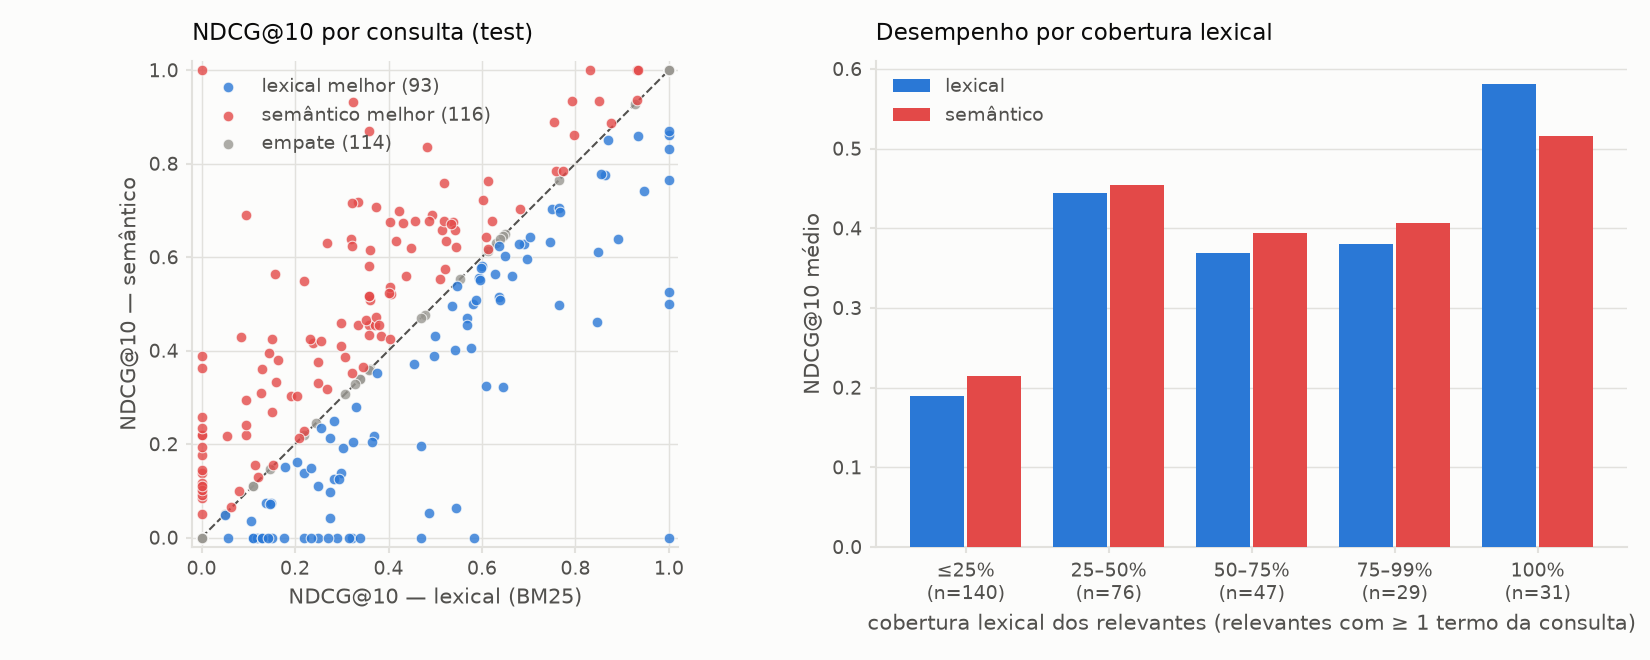
\includegraphics[width=\linewidth]{comparacao_lexical_semantico.png}
\caption{Esquerda: NDCG@10 de cada consulta de test nos dois sistemas (acima da diagonal, semântico melhor). Direita: NDCG@10 médio por faixa de cobertura lexical dos relevantes (fração dos relevantes da consulta que contém ao menos um termo dela).}
\label{fig:lexsem}
\end{figure}

\textbf{Análise por consulta.} As três consultas de maior e as três de menor $\Delta$ foram escolhidas pelo valor, e a Tabela~\ref{tab:seis} mostra o Top-5 de cada sistema com scores e relevantes.

\begin{table}[!htb]
\centering\footnotesize
\caption{As três consultas com maior vantagem de cada sistema (test): Top-5 no formato id (score), sem o prefixo \texttt{MED-}. Relevantes em \textbf{negrito}; \textsuperscript{2} indica grau 2. Scores BM25 e cossenos estão em escalas diferentes e só são comparáveis dentro de cada sistema.}
\label{tab:seis}
\begin{tabularx}{\linewidth}{@{}l c X@{}}
\toprule
Sistema & NDCG@10 & Top-5 \\
\midrule
\multicolumn{3}{@{}l}{\textbf{\pq{1679}}\enspace\emph{myelopathy}\enspace(1 relevante; cobertura lexical 0\%)} \\
Lexical & 0,000 & ranking vazio: \texttt{myelopathi} não existe no índice \\
Semântico & 1,000 & \ri{5142} (0,750)\sep 3316 (0,718)\sep 3317 (0,706)\sep 3288 (0,700)\sep 5135 (0,690) \\
\addlinespace
\multicolumn{3}{@{}l}{\textbf{\pq{307}}\enspace\emph{Vitamin D: Shedding some light on the new recommendations}\enspace(3 relevantes, todos de grau 2)} \\
Lexical & 0,324 & 3099 (14,87)\sep 4872 (14,85)\sep 3373 (12,36)\sep 2180 (11,44)\sep 2765 (11,41) \\
Semântico & 0,933 & \rii{714} (0,800)\sep \rii{919} (0,790)\sep 3990 (0,756)\sep 862 (0,756)\sep 3987 (0,756) \\
\addlinespace
\multicolumn{3}{@{}l}{\textbf{\pq{1537}}\enspace\emph{low-carb diets}\enspace(45 relevantes; cobertura lexical 64\%)} \\
Lexical & 0,095 & 4880 (25,78)\sep 2943 (7,41)\sep 1714 (7,27)\sep \ri{4515} (6,97)\sep 2458 (6,93) \\
Semântico & 0,691 & \ri{4514} (0,817)\sep \ri{1616} (0,812)\sep 4880 (0,812)\sep \ri{4515} (0,811)\sep \ri{2588} (0,810) \\
\midrule
\multicolumn{3}{@{}l}{\textbf{\pq{1473}}\enspace\emph{kohlrabi}\enspace(1 relevante; cobertura lexical 100\%)} \\
Lexical & 1,000 & \ri{4455} (12,59)\enspace(único documento com o termo) \\
Semântico & 0,000 & 4713 (0,589)\sep 5130 (0,577)\sep 1655 (0,562)\sep 4963 (0,559)\sep 4525 (0,555) \\
\addlinespace
\multicolumn{3}{@{}l}{\textbf{\pq{2620}}\enspace\emph{Phytates for the Treatment of Cancer}\enspace(55 relevantes, 19 de grau 2; cobertura lexical 91\%)} \\
Lexical & 0,583 & \ri{2989} (16,59)\sep \rii{4319} (14,21)\sep \ri{2985} (13,83)\sep \rii{2988} (13,64)\sep \ri{2983} (13,29) \\
Semântico & 0,000 & 2435 (0,831)\sep 3551 (0,789)\sep 3548 (0,780)\sep 3555 (0,779)\sep 2922 (0,776) \\
\addlinespace
\multicolumn{3}{@{}l}{\textbf{\pq{2081}}\enspace\emph{shelf life}\enspace(1 relevante; cobertura lexical 100\%)} \\
Lexical & 1,000 & \ri{4303} (17,35)\sep 1182 (12,89)\sep 2700 (12,04)\sep 2671 (10,15)\sep 2074 (8,71) \\
Semântico & 0,500 & 3693 (0,712)\sep 4859 (0,709)\sep \ri{4303} (0,705)\sep 887 (0,696)\sep 4408 (0,679) \\
\bottomrule
\end{tabularx}
\end{table}

\textbf{Semântico superior.}
\begin{itemize}
\item \textbf{\pq{1679} \emph{myelopathy} (termo técnico ausente; paráfrase).} O radical \texttt{myelopathi} não existe no índice (a coleção tem \emph{myelitis}, \emph{myeloma} e \emph{myelin}, mas não \emph{myelopathy}), e o BM25 devolve uma lista vazia. O único relevante, \med{5142}, descreve uma \emph{subacute sclerotic combined degeneration of the spinal cord}; mielopatia é, literalmente, doença da medula espinhal. O bi-encoder liga a consulta ao documento sem nenhuma palavra em comum e o coloca em 1º. É a paráfrase de termo técnico que o Trabalho~1 apontou como limite dos modelos lexicais.
\item \textbf{\pq{307} \emph{Vitamin D: Shedding some light\dots} (expressão idiomática e stopword).} O BM25 lê o idiomatismo literalmente: \texttt{shed} tem idf de 5,60, o maior da consulta, o 1º e o 3º colocados casam \texttt{shed} e \texttt{light}, e quatro dos cinco primeiros contêm \texttt{light}. O 1º (\med{3099}, sobre o receptor aril-hidrocarboneto) e o 3º (\med{3373}, sobre envolvimento social e vizinhança) não têm relação com vitamina D e ocupam as posições 2.691 e 2.834 do semântico. Há também um efeito do pré-processamento: \texttt{d} está na lista de stopwords do NLTK (por contrações como \emph{I'd}), então ``Vitamin D'' vira só \texttt{vitamin} (df $= 222$) e perde a especificidade. O semântico trata a consulta pelo sentido e traz em 1º e 2º os dois relevantes de grau 2 sobre recomendações de vitamina D, que estavam em 21º e 6º no lexical.
\item \textbf{\pq{1537} \emph{low-carb diets} (variação de vocabulário).} A coleção escreve \emph{low-carbohydrate}, não \emph{low-carb}. \texttt{carb} tem df $= 1$, e o único documento que o contém (\med{4880}) não é relevante, mas recebe score 25,8, mais que o triplo do 2º colocado; o resto do ranking lexical é decidido por \texttt{low} e \texttt{diet}, termos genéricos que trazem dietas \emph{low-calorie}, \emph{low-protein} e \emph{low-fat}. O semântico aproxima \emph{carb} de \emph{carbohydrate} e põe 4 relevantes no Top-5, três deles fora do Top-10 lexical (posições 18, 38 e 24).
\end{itemize}

\textbf{Lexical superior.}
\begin{itemize}
\item \textbf{\pq{1473} \emph{kohlrabi} (termo raro com casamento exato).} \texttt{kohlrabi} (couve-rábano) tem df $= 1$, e o único documento que o contém é o relevante: o BM25 acerta em 1º com um único termo. O bi-encoder não tem representação útil para a palavra: o tokenizador a quebra em \texttt{ko \#\#hl \#\#ra \#\#bi}, e o 1º colocado é \emph{A case of Kombucha tea toxicity} (\texttt{ko \#\#mb \#\#uch \#\#a}), seguido de documentos sem relação; o relevante fica em 19º. A maior similaridade dessa consulta é 0,589, a mais baixa entre as seis analisadas (nas outras, de 0,712 a 0,831).
\item \textbf{\pq{2620} \emph{Phytates for the Treatment of Cancer} (termo técnico específico $\times$ generalização).} \texttt{phytat} (df $= 12$, idf de 5,67) ancora o ranking lexical em documentos sobre fitato, e 8 dos 10 primeiros são relevantes. O semântico generaliza para ``compostos alimentares e câncer'' (quimioprevenção, fitoquímicos, flavonoides, frutas vermelhas): tema vizinho, mas sem nenhum relevante no Top-10 (há 10 entre os 50 primeiros). O composto que define a necessidade de informação se dilui no embedding da consulta, ofuscado por \emph{treatment of cancer}.
\item \textbf{\pq{2081} \emph{shelf life} (expressão técnica composta).} \texttt{shelf} (df $= 7$) funciona como etiqueta da expressão, e o BM25 põe o único relevante (\med{4303}, \emph{shelf-life evaluation}) em 1º. O semântico reconhece o tema (armazenamento, oxidação, processamento) e preenche o topo com documentos sobre estocagem de probióticos, de geleia de mirtilo e de hambúrguer, próximos no sentido mas não relevantes; o relevante cai para 3º.
\end{itemize}

\textbf{Padrão.} O lexical vence quando a consulta contém um termo \textbf{raro e específico} que aparece literalmente nos relevantes (\texttt{kohlrabi} com df $= 1$, \texttt{shelf} com 7, \texttt{phytat} com 12): o idf alto transforma o casamento exato num sinal decisivo, enquanto o embedding dilui esse termo numa vizinhança temática. O semântico vence quando consulta e relevantes \textbf{dizem a mesma coisa com palavras diferentes}: termo técnico ausente, variação de forma (\emph{carb}/\emph{carbohydrate}) ou expressão idiomática. É a contrapartida do Trabalho~1: o descasamento de vocabulário que zerava o BM25 lá é justamente o que o bi-encoder resolve aqui, ao custo de perder precisão em termos raros. Ressalva: três das seis consultas têm um único relevante, o que leva o $\Delta$ aos extremos ($\pm 1$); há 23 consultas assim no test.

% ---------------------------------------------------------------------------
\subsection{Tolerância a erros}
\label{sec:res-erros}
% ---------------------------------------------------------------------------

A Tabela~\ref{tab:typo} traz as dez consultas de test nas três condições, no sistema lexical (avaliação obrigatória) e no semântico (opcional). A recuperação é $(\mathrm{NDCG}_{\text{corrigida}} - \mathrm{NDCG}_{\text{erro}}) / (\mathrm{NDCG}_{\text{original}} - \mathrm{NDCG}_{\text{erro}})$, calculada quando o denominador é positivo.

\begin{table}[!htb]
\centering\footnotesize
\setlength{\tabcolsep}{3.5pt}
\caption{Experimento de correção ortográfica: NDCG@10 no test com a consulta original (Orig.), com erro (Erro) e corrigida (Corr.), e recuperação (Recup.) da perda no lexical. Consultas sem o prefixo \texttt{PLAIN-}; o termo com erro está em negrito. ``---'': o erro não reduziu o NDCG@10, e a recuperação não se aplica. A única correção errada é a da consulta 1537 (\emph{low-carb diets}), em que o termo original era \emph{carb}.}
\label{tab:typo}
\begin{tabular}{@{}rlllcccccccc@{}}
\toprule
 & & & & \multicolumn{4}{c}{Lexical (BM25)} & & \multicolumn{3}{c}{Semântico (opcional)} \\
\cmidrule(lr){5-8}\cmidrule(l){10-12}
Consulta & Consulta com erro & Tipo & Correção & Orig. & Erro & Corr. & Recup. & & Orig. & Erro & Corr. \\
\midrule
3312 & Sexually \textbf{Trasnmitted} Fish Toxin & transposição & transmitted & 0,152 & 0,268 & 0,152 & --- & & 0,156 & 0,175 & 0,156 \\
1441 & \textbf{Japam} & substituição & japan & 0,422 & 0,000 & 0,422 & 100\% & & 0,699 & 0,176 & 0,699 \\
1141 & Evidence-based \textbf{medicne} & remoção & medicine & 0,220 & 0,066 & 0,220 & 100\% & & 0,139 & 0,139 & 0,139 \\
56 & Foods for \textbf{Glaucomma} & inserção & glaucoma & 0,679 & 0,000 & 0,679 & 100\% & & 0,627 & 0,625 & 0,627 \\
2030 & \textbf{Rutni} & transposição & rutin & 0,191 & 0,000 & 0,191 & 100\% & & 0,303 & 0,091 & 0,303 \\
1919 & poultry \textbf{wokers} & remoção & workers & 0,797 & 0,407 & 0,797 & 100\% & & 0,860 & 0,212 & 0,860 \\
1847 & \textbf{phillippines} & inserção & philippines & 0,249 & 0,000 & 0,249 & 100\% & & 0,000 & 0,000 & 0,000 \\
1537 & low-\textbf{varb} diets & substituição & \textbf{var} (errada) & 0,095 & 0,095 & 0,073 & --- & & 0,691 & 0,617 & 0,633 \\
541 & American \textbf{Dentak} Association & substituição & dental & 0,179 & 0,000 & 0,179 & 100\% & & 0,151 & 0,000 & 0,151 \\
1419 & \textbf{isnects} & transposição & insects & 0,437 & 0,000 & 0,437 & 100\% & & 0,559 & 0,000 & 0,559 \\
\midrule
\multicolumn{4}{@{}l}{Média (9 de 10 correções exatas)} & 0,342 & 0,084 & 0,340 & 100\% & & 0,419 & 0,204 & 0,413 \\
\bottomrule
\end{tabular}
\end{table}

\begin{itemize}
\item \textbf{O sistema lexical é frágil a um único erro.} Com o erro no termo de maior idf, o NDCG@10 médio cai de 0,3421 para \textbf{0,0836} ($-75{,}6\%$), e 6 das 10 consultas vão a zero. O termo com erro não existe no índice, não tem postings e simplesmente some da consulta. Nas consultas de uma palavra (\emph{Japan}, \emph{Rutin}, \emph{philippines}, \emph{insects}) sobra uma consulta vazia, e em \emph{Foods for Glaucoma} e \emph{American Dental Association} os termos restantes (\texttt{food}, \texttt{american}, \texttt{associ}) são genéricos demais para recuperar algo relevante.
\item \textbf{O corretor recupera 100\% do que foi perdido}: nas 8 consultas em que o erro reduziu o NDCG@10, a correção restaura o termo exato e o NDCG@10 original. As nove correções exatas cobrem os quatro tipos de erro, incluindo as transposições em palavras curtas (\emph{rutni}, \emph{isnects}), o caso mais difícil no dev.
\item \textbf{\pq{3312} \emph{Sexually Transmitted Fish Toxin}: o erro melhorou a consulta.} O título é um trocadilho sobre a ciguatera (toxina de peixe que pode ser transmitida sexualmente), e \texttt{sexual} + \texttt{transmit} puxam para o topo artigos sobre doenças sexualmente transmissíveis (câncer cervical, vaginose bacteriana, HPV), todos não relevantes. Sem \texttt{transmit}, os artigos sobre ciguatera sobem e um relevante de grau 2 (\med{4966}) entra no Top-10 (0,152 $\to$ 0,268); corrigir devolve a consulta original e o seu desempenho. É ambiguidade lexical: o termo existe e casa, mas no sentido errado.
\item \textbf{\pq{1537} \emph{low-carb diets}: a correção errou e piorou.} \emph{varb} está à distância 1 de quatro palavras do dicionário (\emph{var}, \emph{vary}, \emph{carb}, \emph{rarb}), e o desempate pelo Jaccard escolheu \emph{var} (0,50 contra 0,43 de \emph{carb}). \texttt{var} casa com a abreviação botânica \emph{var.}\ (\emph{Actinidia chinensis var.}) e traz artigos sobre kiwi e cereja, derrubando o NDCG@10 para 0,073. O erro em si não tinha custado nada, porque \texttt{carb} tem df $= 1$ e o único documento que o contém nem é relevante. Um corretor sensível ao contexto, que pontuasse a sequência \emph{low-\_\_\_ diets} com estatísticas da coleção, escolheria \emph{carb}; o nosso corrige cada termo isoladamente.
\item \textbf{O semântico é mais robusto, mas não imune} (opcional): ele perde 51,4\% com o erro, contra 75,6\% do lexical, porque o tokenizador WordPiece decompõe o termo com erro em sub-palavras em vez de descartá-lo. \emph{glaucomma} $\to$ \texttt{g \#\#lau \#\#com \#\#ma} mantém o embedding da consulta quase intacto (cosseno de 0,971 com a consulta original), e o NDCG@10 praticamente não muda. Quando os fragmentos perdem a identidade da palavra, o estrago se iguala ao do lexical: \emph{isnects} (\texttt{isn \#\#ect \#\#s}, cosseno de 0,528) e \emph{dentak} vão a zero, \emph{japam} (cosseno de 0,545) cai de 0,699 para 0,176, e \emph{wokers} vira \texttt{woke \#\#rs}, outra palavra real (0,860 $\to$ 0,212). A correção restaura os dois sistemas quase por completo; a diferença residual vem de \emph{varb} $\to$ \emph{var}.
\end{itemize}

% ---------------------------------------------------------------------------
\subsection{Busca híbrida}
\label{sec:res-hibrido}
% ---------------------------------------------------------------------------

A Tabela~\ref{tab:sistemas} e a Figura~\ref{fig:sistemas} comparam os quatro sistemas no test (o reranking é discutido na Seção~\ref{sec:res-rerank}).

\begin{table}[!htb]
\centering\small
\caption{Os quatro sistemas no test (323 consultas), com a variação em relação ao lexical, e o NDCG@10 no dev. Em negrito, o melhor valor de cada coluna.}
\label{tab:sistemas}
\setlength{\tabcolsep}{5pt}
\begin{tabular}{@{}lccccc@{}}
\toprule
Sistema & P@10 & R@10 & MAP@10 & NDCG@10 & NDCG@10 (dev) \\
\midrule
Lexical (BM25) & 0,2402 & 0,1548 & 0,1231 & 0,3300 & 0,2977 \\
Semântico & 0,2567 (+6,8\%) & 0,1620 (+4,6\%) & 0,1230 ($-0{,}1\%$) & 0,3433 (+4,0\%) & 0,3281 \\
Híbrido (RRF) & \textbf{0,2653} (+10,4\%) & \textbf{0,1708} (+10,3\%) & \textbf{0,1395} (+13,3\%) & \textbf{0,3618} (+9,6\%) & \textbf{0,3401} \\
Híbrido + reranking & 0,2505 (+4,3\%) & 0,1688 (+9,1\%) & 0,1391 (+13,0\%) & 0,3564 (+8,0\%) & 0,3341 \\
\bottomrule
\end{tabular}
\end{table}

\begin{figure}[!htb]
\centering
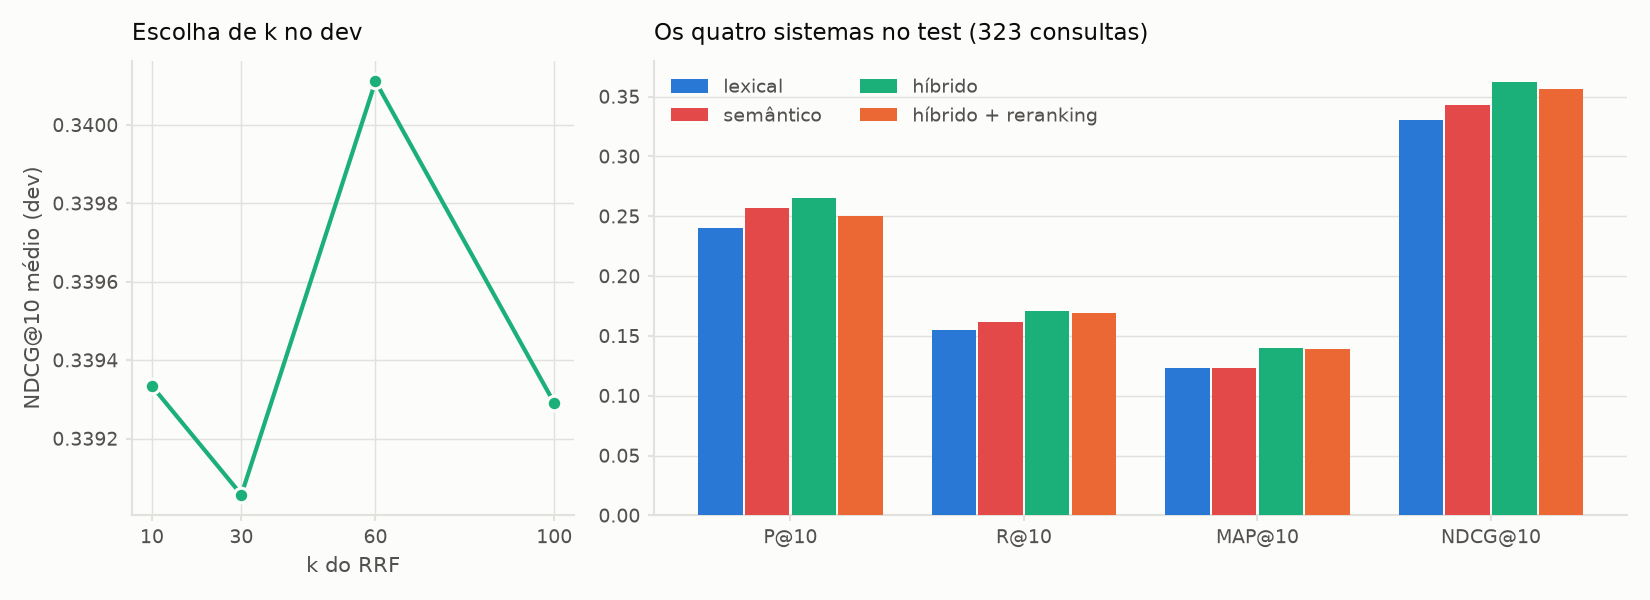
\includegraphics[width=\linewidth]{sistemas_test.png}
\caption{Esquerda: NDCG@10 médio no dev para cada $k$ do RRF (a escala é estreita: a curva varia só 0,001). Direita: as quatro métricas dos quatro sistemas no test.}
\label{fig:sistemas}
\end{figure}

\begin{itemize}
\item \textbf{O valor de $k$ quase não importa.} $k = 60$, o valor proposto no artigo original do RRF (Cormack et al., 2009), venceu no dev, mas a curva é plana (0,3391 a 0,3401): com só dois sistemas e listas de 100 documentos, $k$ quase não muda o resultado.
\item \textbf{O híbrido supera os dois sistemas nas quatro métricas.} No NDCG@10 o ganho é de +9,6\% sobre o lexical e +5,4\% sobre o semântico; no MAP@10, em que os dois empatavam, de +13,3\% e +13,4\%. O ganho já aparecia no dev (0,3401 contra 0,2977 e 0,3281), então não é efeito da escolha de $k$.
\item \textbf{Por que a fusão funciona: complementaridade.} Como os Top-10 dos dois sistemas compartilham só 3,14 documentos em média, cada sistema traz relevantes que o outro não tem. O RRF dá duas contribuições a quem aparece nas duas listas, e \textbf{78,1\%} dos documentos do Top-10 híbrido estão nos dois Top-100: a concordância entre sistemas independentes funciona como evidência adicional de relevância. Dos restantes, 18,9\% vêm só do semântico e 3,0\% só do lexical. A assimetria tem causa estrutural: 127 consultas têm ranking lexical com menos de 100 documentos, enquanto o semântico sempre devolve 100.
\item \textbf{A fusão é segura por consulta.} O híbrido é melhor que os dois sistemas em 60 consultas, iguala o melhor em 138 (77 delas com NDCG@10 $= 0$ nos três), fica entre os dois em 86 e só fica igual ou abaixo do pior em 39 (12\%). Sem saber de antemão qual sistema vai acertar, combinar os dois quase nunca é a pior escolha.
\end{itemize}

% ---------------------------------------------------------------------------
\subsection{Reranking}
\label{sec:res-rerank}
% ---------------------------------------------------------------------------

\textbf{O reranking não melhorou o híbrido: piorou um pouco.} No dev, o NDCG@10 cai de 0,3401 para 0,3341 ($-1{,}8\%$) com o L6 e para 0,3222 ($-5{,}3\%$) com o L12, que é maior. No test, o L6 leva o NDCG@10 de 0,3618 para 0,3564 ($-1{,}5\%$; Tabela~\ref{tab:sistemas}). A perda se concentra no P@10 ($-5{,}6\%$), enquanto o MAP@10 quase não muda (0,1395 $\to$ 0,1391). O resultado continua acima do lexical e do semântico em R@10, MAP@10 e NDCG@10, mas fica abaixo do semântico em P@10.

\textbf{Muita reorganização, efeito líquido quase nulo.} O cross-encoder troca em média 4,47 dos 10 documentos do Top-10, mas o NDCG@10 melhora em 97 consultas, piora em 91 e empata em 135, com $\Delta$ médio de $-0{,}0055$. Para entender o que ele favorece, medimos o deslocamento de todos os pares (consulta, documento) do Top-50 híbrido do test (Tabela~\ref{tab:desloc}).

\begin{table}[!htb]
\centering\small
\caption{Deslocamento médio provocado pelo cross-encoder no Top-50 híbrido do test (posição no híbrido $-$ posição após o reranking; positivo $=$ subiu), por grau e, para os relevantes, pela origem na fusão; e composição dos Top-10 das 323 consultas.}
\label{tab:desloc}
\begin{minipage}[t]{0.33\linewidth}\centering
\begin{tabular}[t]{@{}lrr@{}}
\toprule
Grau & Pares & Desloc. \\
\midrule
2 (citação direta) & 322 & \textbf{+0,56} \\
1 (citação indireta) & 1.659 & \textbf{$-$1,15} \\
0 & 14.169 & +0,12 \\
\bottomrule
\end{tabular}
\end{minipage}\hfill
\begin{minipage}[t]{0.33\linewidth}\centering
\begin{tabular}[t]{@{}lrr@{}}
\toprule
Relevantes & $n$ & Desloc. \\
\midrule
só no lexical & 121 & \textbf{+10,44} \\
só no semântico & 328 & +0,16 \\
nas duas listas & 1.532 & $-$1,98 \\
\bottomrule
\end{tabular}
\end{minipage}\hfill
\begin{minipage}[t]{0.30\linewidth}\centering
\begin{tabular}[t]{@{}lrr@{}}
\toprule
Top-10 & Híbrido & Rerank \\
\midrule
grau 2 & 195 & 198 \\
grau 1 & 662 & 611 \\
não relevantes & 2.373 & 2.421 \\
\bottomrule
\end{tabular}
\end{minipage}
\end{table}

\begin{itemize}
\item \textbf{Ele não é inútil.} Sobe os relevantes de grau 2 e, principalmente, resgata os que só o BM25 tinha encontrado (+10,4 posições), que o RRF subestimava por receberem a contribuição de um único sistema. Lendo consulta e documento juntos, o cross-encoder valoriza a correspondência textual explícita, o que é coerente com seu treino no MS MARCO (trechos da web que respondem a consultas do Bing).
\item \textbf{Mas rebaixa os relevantes de grau 1}, que são a maioria (1.659 contra 322 de grau 2 no Top-50), e os documentos que estavam nas duas listas, justamente os que o RRF tinha promovido por consenso. No Top-10, os de grau 2 passam de 195 para 198, os de grau 1 caem de 662 para 611 e os não relevantes sobem de 2.373 para 2.421: é isso que derruba o P@10. O NDCG@10 cai menos porque o grau 2 vale o dobro e aumenta.
\item \textbf{Hipótese: descasamento entre o critério do modelo e o dos qrels.} No MS MARCO, relevante é o trecho que \emph{responde} à pergunta; no NFCorpus, é o estudo \emph{citado} por um artigo sobre o tema, e o grau 1 (citação indireta) marca justamente documentos relacionados ao tema que não necessariamente respondem à consulta. O L12, mais especializado no MS MARCO, perde mais no dev, o que é coerente com a hipótese, mas não a prova.
\end{itemize}

\textbf{Os quatro casos.} Selecionados pela diferença $\Delta = \mathrm{NDCG@10}_{\text{rerank}} - \mathrm{NDCG@10}_{\text{híbrido}}$: os dois maiores ganhos; entre as consultas com $|\Delta| < 0{,}005$ e NDCG@10 híbrido maior que zero, a de mais relevantes no Top-10 híbrido (um caso em que o híbrido já acertava); e a maior perda. A Tabela~\ref{tab:rerankcasos} mostra os principais documentos que mudaram de posição.

\begin{table}[!htb]
\centering\footnotesize
\caption{Principais documentos que mudaram de posição nos quatro casos de reranking (test). CE $=$ score do cross-encoder; grau 0 $=$ não julgado. Títulos abreviados.}
\label{tab:rerankcasos}
\begin{tabularx}{\linewidth}{@{}l c c r >{\raggedright\arraybackslash}X@{}}
\toprule
Documento & Grau & Híbrido $\to$ rerank & CE & Título \\
\midrule
\multicolumn{5}{@{}l}{\textbf{Maior ganho: \pq{2281}} \emph{turnips}\enspace NDCG@10 0,000 $\to$ 0,431 (1 relevante)} \\
\med{2098} & 1 & 45 $\to$ 4 & $-$7,89 & Steam cooking significantly improves in vitro bile acid\dots \\
\med{2066} & 0 & 2 $\to$ 1 & $-$0,99 & Glucosinolates in Brassica vegetables\dots \\
\med{3370} & 0 & 4 $\to$ 41 & $-$10,63 & Serving styles of raw snack vegetables\dots \\
\med{3374} & 0 & 5 $\to$ 49 & $-$11,13 & Attractive names sustain increased vegetable intake in\dots \\
\addlinespace
\multicolumn{5}{@{}l}{\textbf{Segundo maior ganho: \pq{1320}} \emph{Harvard Physicians' Study II}\enspace NDCG@10 0,196 $\to$ 0,562 (6 relevantes)} \\
\med{2760} & 1 & 7 $\to$ 1 & 0,18 & Multivitamins in the Prevention of Cancer in Men: The Physicians' Health Study II \\
\med{4929} & 0 & 4 $\to$ 2 & $-$0,26 & Vitamins E and C in the Prevention of Cardiovascular Disease in Men: The Physicians' Health Study II \\
\med{2758} & 1 & 8 $\to$ 3 & $-$1,95 & Multivitamins in the Prevention of Cardiovascular Disease in Men: The Physicians' Health Study II \\
\med{2761} & 1 & 26 $\to$ 6 & $-$5,36 & Who uses multivitamins? A cross-sectional study in the Physicians' Health Study \\
\med{1545} & 0 & 1 $\to$ 21 & $-$8,98 & Physician smoking status, attitudes toward smoking\dots \\
\med{1549} & 0 & 2 $\to$ 15 & $-$7,91 & Physicians' health habits are associated with lifestyle counseling\dots \\
\addlinespace
\multicolumn{5}{@{}l}{\textbf{Pouca alteração: \pq{1398}} \emph{IGF-1}\enspace NDCG@10 1,000 $\to$ 1,000 (103 relevantes, todos de grau 1)} \\
\med{1722} & 1 & 3 $\to$ 1 & 6,55 & Insulin-like growth factor-1 and childhood cancer risk \\
\med{4216} & 1 & 12 $\to$ 3 & 5,27 & Relationship of dietary protein and soy isoflavones to\dots \\
\med{4228} & 1 & 1 $\to$ 11 & 3,54 & Circulating insulin-like growth factor (IGF) peptides\dots \\
\med{1716} & 1 & 7 $\to$ 24 & 0,14 & A Twenty-First Century Cancer Epidemic Caused by Obesity\dots \\
\addlinespace
\multicolumn{5}{@{}l}{\textbf{Maior perda: \pq{1679}} \emph{myelopathy}\enspace NDCG@10 1,000 $\to$ 0,000 (1 relevante)} \\
\med{1105} & 0 & 41 $\to$ 1 & 0,44 & A case of multiple myeloma presenting as a bullous dermatosis \\
\med{1109} & 0 & 39 $\to$ 3 & $-$3,82 & Risk factors for multiple myeloma\dots \\
\med{5142} & 1 & 1 $\to$ 42 & $-$10,20 & Irreversible subacute sclerotic combined degeneration of the spinal cord\dots \\
\bottomrule
\end{tabularx}
\end{table}

\begin{itemize}
\item \textbf{\pq{2281} \emph{turnips} (0,000 $\to$ 0,431).} O único relevante (\med{2098}) sobe do 45º para o 4º lugar. Ele não menciona \emph{turnip}: trata do cozimento a vapor de couve, kale, folhas de mostarda, brócolis e repolho, crucíferas como o nabo, e por isso nem aparece no ranking lexical. O Top-10 híbrido vinha dominado por documentos genéricos sobre vegetais trazidos pelo semântico (1º e 2º no semântico), que o cross-encoder manda para o 41º e o 49º; em 1º ele põe um artigo sobre glucosinolatos em vegetais do gênero \emph{Brassica}, a família do nabo. Porém \textbf{todos os scores são negativos} (o maior é $-0{,}99$): o modelo não considera nenhum candidato uma boa resposta, e o ganho vem de uma reordenação entre candidatos fracos que, desta vez, favoreceu o relevante.
\item \textbf{\pq{1320} \emph{Harvard Physicians' Study II} (0,196 $\to$ 0,562).} A consulta nomeia um ensaio clínico, o \emph{Physicians' Health Study II}. No híbrido, o Top-10 era tomado por documentos sobre médicos (tabagismo e hábitos de saúde de médicos): lexical e semântico trataram \emph{physician} como o tema da consulta. O cross-encoder reconhece a entidade e sobe os artigos do próprio estudo (7º $\to$ 1º, 8º $\to$ 3º e 26º $\to$ 6º). O 2º colocado após o reranking (\med{4929}) também é um artigo do estudo, mas \textbf{não está nos qrels}: o NDCG@10 de 0,562 subestima o acerto, um exemplo concreto de qrels incompletos.
\item \textbf{\pq{1398} \emph{IGF-1} (1,000 $\to$ 1,000).} São 103 relevantes, todos de grau 1, e o Top-10 híbrido já era 100\% relevante. O cross-encoder o reorganiza bastante (o antigo 1º cai para 11º, e quatro documentos saem do Top-10), mas os que entram também são relevantes de grau 1. Com todos os relevantes no mesmo grau, o NDCG@10 é indiferente à ordem entre eles: a métrica satura. Aqui os scores são altos e positivos nos dez primeiros (3,6 a 6,6), porque a entidade da consulta aparece literalmente nos títulos (\emph{Insulin-like growth factor-1\dots}).
\item \textbf{\pq{1679} \emph{myelopathy} (1,000 $\to$ 0,000).} O caso que o bi-encoder tinha resolvido na Seção~\ref{sec:res-lexsem} é desfeito. O relevante \med{5142} (degeneração da medula espinhal) cai do 1º para o 42º lugar, com score de $-10{,}2$, entre os mais baixos dos 50. Em 1º e em 3º o cross-encoder põe artigos sobre \emph{multiple myeloma}: mieloma compartilha com mielopatia o radical \emph{myel-} (medula), mas é um câncer da medula \emph{óssea}. O cross-encoder trocou a paráfrase correta por semelhança de superfície, coerente com o ganho que ele dá aos relevantes encontrados só pelo lexical.
\end{itemize}

\textbf{Síntese.} O cross-encoder acerta quando a consulta tem uma entidade explícita que o texto do documento confirma (\emph{Physicians' Health Study II}, \emph{IGF-1}) e erra quando a relevância depende de conhecimento de domínio que ele não tem (mielopatia $\neq$ mieloma) ou de uma noção temática de relevância diferente da do seu treino. Um reranker mais preciso \emph{em geral} não é automaticamente melhor \emph{nesta coleção}; por isso ele foi avaliado no dev, e não presumido.

% ---------------------------------------------------------------------------
\subsection{Tempos}
% ---------------------------------------------------------------------------

\begin{table}[!htb]
\centering\small
\caption{Custo das etapas em CPU (Intel Core i5-1340P). Tempos por consulta medidos nas 323 consultas de test.}
\label{tab:tempos}
\begin{tabular}{@{}lrl@{}}
\toprule
Etapa & Tempo & Observação \\
\midrule
\multicolumn{3}{@{}l}{\emph{Pré-cálculo (uma vez)}} \\
Pré-processamento da coleção & 0,35 s & \texttt{stopwords+stemming} \\
Construção do índice invertido & 0,21 s & média de 5 construções \\
Embeddings dos 3.633 documentos & 539 s & \texttt{bge-small-en-v1.5} \\
\midrule
\multicolumn{3}{@{}l}{\emph{Por consulta (média)}} \\
Lexical (BM25) & 0,44 ms & pré-processamento, acúmulo e ordenação \\
Semântica & 132,64 ms & 125,30 ms de codificação + 7,34 ms de busca exaustiva \\
Fusão (RRF) & 0,11 ms & \\
Reranking (50 pares) & 4.112,99 ms & 96,9\% do total; o L12 levava 8,61 s no dev \\
\textbf{Total da recuperação} & \textbf{4.246,19 ms} & \\
\midrule
\multicolumn{3}{@{}l}{\emph{Geração (média por resposta)}} \\
LLM, condição A & 17 s & prompt de até 52 tokens \\
LLM, condição B & 26 s & prompt de 1.544 a 2.943 tokens \\
\bottomrule
\end{tabular}
\end{table}

A Tabela~\ref{tab:tempos} resume os custos. \textbf{O reranking domina o custo da recuperação}: o cross-encoder faz uma passada do transformer \emph{por par}, 50 por consulta, e responde por 97\% do tempo do pipeline; em CPU, é ele que limita a profundidade do reordenamento (reordenar 100 documentos dobraria esse tempo). O semântico é cerca de 300$\times$ mais caro por consulta que o BM25, mas o custo está na rede neural, não na busca: a busca exaustiva em si leva 7,3 ms e poderia continuar exaustiva numa coleção bem maior. Os embeddings dos documentos levam 539 s, contra 0,21 s para construir o índice invertido. Na geração, a condição B leva 9 s a mais por resposta, sobretudo pelo processamento dos cerca de 2.000 tokens de contexto; somando recuperação e reranking, o pipeline completo responde uma pergunta em cerca de meio minuto. O tempo lexical foi medido com $k_1 = 1{,}2$ e $b = 0{,}75$, já que os parâmetros não alteram o custo.

% ---------------------------------------------------------------------------
\subsection{RAG}
\label{sec:res-rag}
% ---------------------------------------------------------------------------

A Tabela~\ref{tab:ragq} reúne, para as dez consultas, a recuperação (o que chegou à LLM) e a nota humana de cada condição; a Tabela~\ref{tab:ragnotas} traz as médias por critério e a concordância entre os avaliadores.

\begin{table}[!htb]
\centering\small
\caption{RAG por consulta. ``Rel.'': relevantes da consulta nos qrels; recuperação medida sobre os 5 documentos enviados à LLM; ``A'' e ``B'': média de fidelidade, completude e utilidade (média dos dois avaliadores), os três critérios comuns às duas condições.}
\label{tab:ragq}
\setlength{\tabcolsep}{5pt}
\begin{tabular}{@{}llccccccc@{}}
\toprule
Consulta & Pergunta & Rel. & P@5 & R@5 & Hit@5 & A & B & B $-$ A \\
\midrule
\pq{68}   & What is Actually in Chicken Nuggets?          & 55 & 0,2 & 0,018 & 1 & 0,50 & 2,00 & \textbf{+1,50} \\
\pq{2450} & Are Organic Foods Safer?                      & 38 & 0,4 & 0,053 & 1 & 1,33 & 1,33 & 0,00 \\
\pq{153}  & How Should I Take Probiotics?                 & 47 & 1,0 & 0,106 & 1 & 0,67 & 2,00 & +1,33 \\
\pq{2850} & More Antibiotics In White Meat or Dark Meat?  &  9 & 0,0 & 0,000 & \textbf{0} & 0,67 & 1,17 & +0,50 \\
\pq{2750} & Preventing the Common Cold with Probiotics?   & 59 & 0,8 & 0,068 & 1 & 0,67 & 1,67 & +1,00 \\
\pq{270}  & Is Caffeinated Tea Really Dehydrating?        & 52 & 0,4 & 0,038 & 1 & 1,17 & 2,00 & +0,83 \\
\pq{2470} & Is Milk Good for Our Bones?                   & 73 & 0,6 & 0,041 & 1 & 0,50 & 1,33 & +0,83 \\
\pq{2430} & Preventing Brain Loss with B Vitamins?        & 46 & 0,6 & 0,065 & 1 & 1,00 & 1,33 & +0,33 \\
\pq{238}  & How Chemically Contaminated Are We?           & 54 & 0,2 & 0,019 & 1 & 1,00 & 1,50 & +0,50 \\
\pq{3342} & Is Coconut Milk Good For You?                 &  3 & 0,2 & 0,333 & 1 & 1,00 & 1,00 & 0,00 \\
\midrule
Média & & 43,6 & \textbf{0,44} & \textbf{0,074} & \textbf{0,9} & 0,85 & \textbf{1,53} & +0,68 \\
\bottomrule
\end{tabular}
\end{table}

\begin{table}[!htb]
\centering\small
\caption{Avaliação humana: médias por critério e condição (nota de cada critério $=$ média dos dois avaliadores) e concordância entre os avaliadores ($n = 20$ respostas; na rastreabilidade, só as 10 da condição B).}
\label{tab:ragnotas}
\begin{tabular}{@{}lcccc@{}}
\toprule
Critério & A (sem RAG) & B (com RAG) & Notas idênticas & Kappa ponderado \\
\midrule
Fidelidade      & 0,65 & \textbf{1,45} & 60\% & 0,497 \\
Completude      & 1,05 & \textbf{1,55} & 40\% & 0,333 \\
Utilidade       & 0,85 & \textbf{1,60} & 55\% & 0,444 \\
Rastreabilidade & N/A  & 1,35 & 90\% & 0,783 \\
\midrule
Média (fidelidade, completude, utilidade) & 0,85 & \textbf{1,53} & & \\
\bottomrule
\end{tabular}
\end{table}

\textbf{Recuperação: o que chegou à LLM.} Em \textbf{9 das 10} consultas ao menos um documento relevante chegou à LLM (Hit@5 $= 0{,}9$), e em média 2,2 dos 5 documentos do contexto são relevantes (P@5 $= 0{,}44$). O R@5 baixo (0,074) é consequência do número de relevantes, como o enunciado antecipa: com dezenas de relevantes por consulta, o R@5 máximo possível fica entre 0,07 e 0,13 em 8 das 10 consultas (a média do máximo nas dez é 0,23, puxada pela \pq{3342}, com 3 relevantes, e pela \pq{2850}, com 9). A exceção é a \pq{2850}, em que \emph{nenhum} relevante chegou ao contexto (Seção~\ref{sec:res-falhas}).

\textbf{O que muda, objetivamente, nas respostas.} As respostas com RAG citam em média 2,5 documentos distintos, 1,3 deles relevantes nos qrels, e \textbf{nenhum id citado está fora do contexto}: a LLM não inventou fontes. As respostas sem RAG não citam nada. As respostas com RAG são um pouco mais curtas (205 contra 224 palavras; o limite de 200 palavras foi excedido nas duas condições) e declaram explicitamente a limitação da evidência com mais frequência (7 de 10, contra nenhuma sem RAG, por uma heurística de expressões como \emph{limited}, \emph{not directly addressed} e \emph{further research}).

\textbf{O RAG melhorou as respostas nos três critérios comuns}, e o maior ganho foi na \textbf{fidelidade} (0,65 $\to$ 1,45). Ele melhorou em 8 das 10 consultas, empatou em 2 e não piorou em nenhuma. O resultado não depende de um avaliador: separadamente, a média dos três critérios vai de 1,10 para 1,60 para o primeiro avaliador e de 0,60 para 1,47 para o segundo, e em nenhum item os dois divergiram em mais de 1 ponto. A concordância é alta na rastreabilidade, o critério mais objetivo (há ou não um \texttt{doc\_id} que sustente a afirmação), e moderada nos demais.

\textbf{Sem contexto, a LLM repete o senso comum, mesmo quando a evidência diz o contrário.} As notas de fidelidade da condição A são as mais baixas porque várias respostas contradizem os documentos recuperados:
\begin{itemize}
\item \pq{68}: descreve os nuggets como carne de peito ou coxa empanada, mas o \med{2991} conclui que o músculo não é o componente predominante e que eles são majoritariamente gordura.
\item \pq{153}: manda tomar probióticos em jejum, longe das refeições, mas o \med{3679} conclui que a sobrevivência é melhor com a refeição ou até 30 minutos antes.
\item \pq{2470}: afirma que \emph{``milk is indeed good for our bones''}, mas nenhum dos três estudos encontra redução de fraturas, e o \med{1338} encontra mais fraturas em mulheres.
\item \pq{270}: sugere compensar o chá com água, mas o \med{4331} não encontra diferença de hidratação em relação à água.
\item \pq{2750}: conclui que os probióticos \emph{``may not prevent the common cold''}, mas o \med{3683} e o \med{3680} mostram redução da incidência.
\end{itemize}
Várias dessas perguntas questionam justamente uma crença comum (\emph{Is Caffeinated Tea \textbf{Really} Dehydrating?}, \emph{What is \textbf{Actually} in Chicken Nuggets?}), e é nelas que a resposta paramétrica de um modelo pequeno reproduz a crença.

\textbf{Com contexto, os erros mudam de natureza: de crença sem fonte para leitura errada de uma fonte.} A fidelidade média da condição B (1,45) ainda está longe de 2. Os erros apontados pelos dois avaliadores são de interpretação e atribuição: menor contaminação bacteriana nos orgânicos, quando o \med{1178} diz que ela não depende do método de cultivo (\pq{2450}); o achado de HDL do \med{4000} atribuído ao \med{5014} (\pq{3342}); carne escura tratada como carne bovina (\pq{2850}). Também há o uso de documentos fora do tema que estavam no contexto: vitaminas E e C (\med{4929}) numa pergunta sobre vitaminas B, e chá com leite e função vascular (\med{4902}) numa pergunta sobre ossos. Com P@5 $= 0{,}44$, mais da metade do contexto não é relevante, e o modelo de 3 bilhões de parâmetros tende a usar tudo o que recebe.

\textbf{Rastreabilidade: o que a ausência de fontes esconde.} Na condição A a rastreabilidade é N/A: nenhuma afirmação pode ser conferida, inclusive números e mecanismos que não estão em nenhum documento e soam confiáveis (\emph{1--2 billion CFU}, \emph{MCTs reduce bad cholesterol}). Na condição B (1,35), as citações nunca apontam para documentos fora do contexto, mas nem sempre sustentam a afirmação a que estão presas. A diferença prática é que os erros da condição B são \textbf{detectáveis}: foi justamente pelas citações que os dois avaliadores identificaram as atribuições trocadas, enquanto os erros da condição A só aparecem para quem já conhece a literatura.

\textbf{Limites da avaliação.} A completude tem a menor concordância (40\% de notas idênticas, $\kappa = 0{,}33$), e as justificativas mostram duas leituras da rubrica: o primeiro avaliador mediu a cobertura dos aspectos da pergunta em geral, e as respostas sem RAG, longas e abrangentes, receberam 2 em 4 dos 10 casos; o segundo mediu a cobertura do que os documentos permitem responder, e sua média de completude na condição A é 0,7, contra 1,4 do primeiro. A rubrica fala nos aspectos ``que podem ser respondidos'', o que favorece a segunda leitura, mas a conclusão de que B $>$ A vale nas duas. Além disso, as citações \texttt{[MED-\dots]} identificam as respostas da condição B, e as da condição A, longas e genéricas, também são reconhecíveis: a avaliação não foi de fato cega quanto à condição, o que pode ter ampliado a diferença. O efeito é atenuado pela exigência de justificar cada nota com base em documentos específicos: as notas baixas da condição A vêm acompanhadas da contradição concreta com o documento.

% ---------------------------------------------------------------------------
\subsection{Análise de falhas ponta a ponta}
\label{sec:res-falhas}
% ---------------------------------------------------------------------------

Para localizar onde a evidência se perde, seguimos os documentos relevantes de cada consulta ao longo do pipeline (Tabela~\ref{tab:trace}): se nenhum relevante chega ao Top-50 híbrido, o problema está na recuperação; se chega ao Top-50 mas não ao Top-5, no reranking ou na seleção de contexto; se chega ao Top-5, na geração.

\begin{table}[!htb]
\centering\small
\caption{Número de documentos relevantes em cada estágio do pipeline, nas dez consultas do RAG. O Top-50 híbrido é o conjunto que o cross-encoder vê; o Top-5 é o que a LLM recebe.}
\label{tab:trace}
\begin{tabular}{@{}lccccccc@{}}
\toprule
Consulta & Relevantes & \makecell{Lexical\\Top-100} & \makecell{Semântico\\Top-100} & \makecell{Em ao menos\\um dos dois} & \makecell{Híbrido\\Top-50} & \makecell{Contexto\\Top-5} & \makecell{Grau 2 no\\contexto} \\
\midrule
\pq{68}   & 55 & 12 & 14 & 22 &  9 & 1 & 1 \\
\pq{2450} & 38 &  7 &  7 &  8 &  6 & 2 & 2 \\
\pq{153}  & 47 & 17 & 22 & 23 & 18 & 5 & 1 \\
\pq{2850} &  9 &  2 &  4 &  4 &  1 & \textbf{0} & 0 \\
\pq{2750} & 59 & 16 & 24 & 25 & 17 & 4 & 2 \\
\pq{270}  & 52 & 13 &  9 & 15 &  4 & 2 & 0 \\
\pq{2470} & 73 & 26 & 20 & 28 & 18 & 3 & 3 \\
\pq{2430} & 46 & 11 & 18 & 19 & 16 & 3 & 3 \\
\pq{238}  & 54 &  3 &  2 &  4 &  2 & 1 & 0 \\
\pq{3342} &  3 &  3 &  3 &  3 &  3 & 1 & 1 \\
\midrule
Total & 436 & 110 & 123 & 151 & 94 & 22 & 13 \\
\bottomrule
\end{tabular}
\end{table}

\textbf{O gargalo principal é a primeira etapa.} Dos 436 relevantes das dez consultas, 151 estão no Top-100 de ao menos um sistema; os outros \textbf{285 (65\%)} não aparecem em nenhum dos rankings iniciais e nunca têm chance de chegar ao contexto, o que é coerente com a cobertura lexical de 39\% medida na Seção~\ref{sec:res-lexsem}. A fusão leva 94 dos 151 ao Top-50, e daí em diante o Top-5 é um corte de 1/10 do Top-50, então é natural que a maior parte dos relevantes do Top-50 fique de fora.

\textbf{Seleção dos casos pelas notas humanas.} A diferença B $-$ A na média dos três critérios comuns define os casos: a maior diferença (o RAG melhorou claramente), \pq{68} (+1,50); a menor diferença (o RAG não ajudou ou prejudicou), com empate decidido pela pior nota da resposta com RAG, \pq{3342} (0,00; B $= 1{,}00$); e, entre as demais, a de menor diferença em módulo (pouca diferença), \pq{2450} (0,00). Nenhuma consulta piorou com o RAG. Analisamos também a \pq{2850}, a única sem relevante no contexto. A Tabela~\ref{tab:casosrag} segue o documento-chave de cada caso pelo pipeline.

\begin{table}[!htb]
\centering\small
\caption{Trajetória dos documentos-chave nos casos analisados: posição em cada estágio e estágio em que o problema ocorreu. ``---'': fora do ranking lexical; \textsuperscript{*}fora do Top-50 híbrido, que é o que o cross-encoder reordena (a posição não muda).}
\label{tab:casosrag}
\begin{tabularx}{\linewidth}{@{}l l c c c c >{\raggedright\arraybackslash}X@{}}
\toprule
Consulta (B $-$ A) & Documento (grau) & Lexical & Semântico & Híbrido & Rerank & Estágio do problema \\
\midrule
\pq{68} (+1,50)   & \med{2991} (2) & 1 & 1 & 1 & 1 & nenhum: o RAG corrige a crença comum \\
\addlinespace
\pq{2450} (0,00)  & \med{1178} (2) & 2 & 2 & 2 & 2 & geração: leitura errada de uma frase com nuance \\
\addlinespace
\pq{3342} (0,00)  & \med{5014} (2) & 2 & 2 & 1 & 1 & geração, com contexto poluído pelo reranking \\
                  & \med{5039} (0) & --- & 11 & 46 & 4 & \\
\addlinespace
\pq{2850} (+0,50) & \med{4166} (2) & 174 & 33 & 76 & 76\textsuperscript{*} & recuperação lexical + fusão: o cross-encoder nunca viu o documento \\
                  & \med{4167} (1) & 76 & 46 & 36 & 10 & \\
\bottomrule
\end{tabularx}
\end{table}

\textbf{\pq{68} \emph{What is Actually in Chicken Nuggets?}: o RAG melhorou claramente} (A: 0,5 nos três critérios; B: 2 nos quatro, para os dois avaliadores). O documento que responde à pergunta, \med{2991} (\emph{The autopsy of chicken nuggets reads ``chicken little''}, grau 2), é o 1º colocado em \emph{todos} os estágios. A resposta B o resume com fidelidade (predomínio de gordura, músculo não predominante, epitélio, osso, nervo, tecido conjuntivo, ``o nome é enganoso'') e ignora os outros quatro documentos do contexto, todos não relevantes (genética de frangos, arsênico em frango, adenovírus e adiposidade, estresse por superlotação). A resposta A descreve nuggets como carne de peito ou coxa empanada, exatamente o que o estudo desmente. O RAG funciona melhor quando o documento decisivo está no topo e é autoexplicativo: mesmo com P@5 $= 0{,}2$, um único documento bastou, e o ruído do contexto não contaminou a resposta.

\textbf{\pq{2450} \emph{Are Organic Foods Safer?}: pouca diferença} (A e B com 1,0 em fidelidade e 1,5 em completude e utilidade). As duas respostas chegam à mesma conclusão geral (orgânico não é automaticamente mais seguro) por caminhos diferentes. A resposta A é genérica e se contradiz: diz que orgânicos são ``geralmente considerados mais seguros'' e, na frase seguinte, que não são. A resposta B se apoia nos documentos, mas lê errado o achado central do \med{1178} (2º no contexto, grau 2): afirma que há menos contaminação bacteriana nos orgânicos, quando o estudo diz que ela não depende do método de cultivo, e omite o que de fato difere, as bactérias resistentes a antibióticos. \textbf{Estágio do problema: geração.} A informação certa estava no contexto e foi mal interpretada. O RAG não mudou a nota, mas mudou o tipo de erro: de uma generalidade sem fonte para uma leitura errada verificável (rastreabilidade 1 em B, N/A em A).

\textbf{\pq{3342} \emph{Is Coconut Milk Good For You?}: o RAG não ajudou} (A: fidelidade 0,5, completude 1,5 e utilidade 1,0; B: 1,0 nos quatro critérios). A resposta B ganha em fidelidade, porque deixa de afirmar sem base que a gordura do leite de coco reduz o LDL, mas perde em completude. O rastreamento localiza o problema:
\begin{itemize}
\item \textbf{Recuperação, fusão e reranking não falharam para o documento-chave.} O \med{5014} (grau 2) é o 2º no lexical e no semântico e o 1º no híbrido e após o reranking. Ele traz a evidência direta sobre a pergunta: \emph{``Coconut consumption as flesh or milk was not different between cases and controls''}, e a gordura saturada do coco não foi preditora de doença coronariana.
\item \textbf{A composição do contexto atrapalhou.} Os outros quatro documentos não são relevantes nos qrels: dois tratam de \emph{óleo} de coco (\med{4000}, \med{4002}), um de \emph{água} de coco intravenosa (\med{5015}) e um de \emph{cacau} (\med{5039}, \emph{Cocoa and cardiovascular health}). Este último nem aparece no ranking lexical, era o 46º no híbrido e foi promovido pelo cross-encoder para o 4º lugar: é a mesma confusão de superfície (\emph{coconut} $\times$ \emph{cocoa}) que a Seção~\ref{sec:res-rerank} encontrou em \emph{myelopathy} $\times$ \emph{myeloma}.
\item \textbf{A geração falhou com a informação disponível.} A resposta B afirma que os estudos \emph{``focus on coconut oil and not coconut milk''} e que os efeitos do leite de coco \emph{``are not directly addressed''}, o que é falso diante do \med{5014}; além disso, atribui ao \med{5014} o aumento de HDL em mulheres filipinas, achado do \med{4000}. Os dois avaliadores apontaram as duas falhas.
\end{itemize}
\textbf{Estágio do problema: geração, agravada pela seleção de contexto.} A informação necessária chegou ao contexto, em 1º lugar, mas o modelo foi atraído pela maioria de documentos sobre óleo de coco, generalizou a partir deles e deixou de ler o achado sobre leite de coco no documento certo. Um contexto mais limpo, sem os documentos sobre água de coco e cacau que o reranker promoveu, ou um modelo maior, mais capaz de separar óleo de leite, poderiam ter evitado a falha. Não é um caso de ``a LLM errou'' isoladamente: o reranking contribuiu com ruído.

\textbf{\pq{2850} \emph{More Antibiotics In White Meat or Dark Meat?}: a evidência não chegou ao contexto} (Hit@5 $= 0$).
\begin{itemize}
\item O relevante de grau 2, \med{4166} (\emph{Concentrations of antibiotic residues vary between different edible muscle tissues in poultry}), responde exatamente à pergunta, mas fala em \emph{muscle tissues}, não em \emph{white meat} ou \emph{dark meat}: o BM25 o coloca só em 174º, e o semântico, em 33º.
\item Por ficar fora do Top-100 lexical, ele recebe do RRF a contribuição de um único sistema e cai para o 76º lugar no híbrido, fora do Top-50: \textbf{o cross-encoder nunca chega a vê-lo}. O único relevante que entra no Top-50 (\med{4167}, sobre ingestão inadvertida de antibióticos) termina em 10º após o reranking.
\item Os cinco documentos enviados à LLM tratam de resistência antimicrobiana em carnes do varejo, bacteriófagos em produtos cárneos, consumo de carne e mortalidade e câncer colorretal: são do tema ``carne'', sem relação com a comparação entre carne branca e escura, e todos têm score negativo no cross-encoder ($-5{,}0$ a $-6{,}1$), ou seja, o reranker não encontrou nenhum candidato convincente.
\end{itemize}
\textbf{Estágio do problema: recuperação lexical somada à fusão.} O descasamento de vocabulário (\emph{white/dark meat} $\times$ \emph{muscle tissues}) tirou o documento do ranking lexical, e o RRF, que recompensa a concordância entre os sistemas, rebaixou um documento que só o semântico tinha encontrado; usando só o semântico, ele estaria em 33º, ao alcance do cross-encoder. Como a informação necessária não chegou ao contexto, a falha é anterior à geração: nenhuma melhoria da LLM resolveria este caso.

\textbf{Síntese ponta a ponta.} Quando o documento certo chega ao contexto, o RAG melhora ou empata; os empates vêm da geração de um modelo pequeno, que lê mal uma frase com nuance ou se deixa levar pela maioria dos documentos do contexto. Quando o documento não chega, a falha está na recuperação.

% ===========================================================================
\section{Considerações Finais}
% ===========================================================================

\begin{enumerate}
\item \textbf{Lexical e semântico são complementares, e a fusão é a intervenção que mais rende.} Os Top-10 dos dois sistemas têm só 3,14 documentos em comum; o lexical vence com termos raros e exatos (\emph{kohlrabi}, df $= 1$), e o semântico com paráfrase e variação de vocabulário (\emph{myelopathy}, \emph{low-carb}). O RRF supera os dois sistemas nas quatro métricas (+9,6\% de NDCG@10 sobre o BM25 e +5,4\% sobre o semântico) e fica igual ou abaixo do pior sistema em só 12\% das consultas.
\item \textbf{Um modelo ``mais preciso'' em geral não é automaticamente melhor nesta coleção.} O cross-encoder treinado no MS MARCO ($-1{,}5\%$ de NDCG@10 no test; o L12, $-5{,}3\%$ no dev) e o bi-encoder treinado em pares pergunta-resposta ($-8{,}2\%$ em relação ao BM25 no dev) pioram numa coleção cuja relevância é temática, definida por citações. O cross-encoder reorganiza muito o topo (4,47 de 10 documentos trocados), resgata relevantes que só o lexical tinha encontrado, mas rebaixa os de grau 1 e se deixa levar por semelhança de superfície (\emph{myelopathy} $\times$ \emph{myeloma}, \emph{coconut} $\times$ \emph{cocoa}). Só a validação no dev revelou isso.
\item \textbf{A busca lexical é frágil a erros ortográficos, e a correção por k-gramas resolve o erro isolado.} Um único erro no termo de maior idf derruba o NDCG@10 em 76\% e zera 6 de 10 consultas; o corretor recupera 100\% da perda nas 8 consultas afetadas. O semântico é mais robusto ($-51\%$), mas não imune. O limite do corretor é o desempate sem contexto (\emph{varb} $\to$ \emph{var}).
\item \textbf{O RAG melhora as respostas quando a evidência chega ao contexto, e o gargalo é a primeira etapa da recuperação.} A fidelidade vai de 0,65 para 1,45, o RAG melhora 8 das 10 respostas e não piora nenhuma, e as citações tornam os erros restantes verificáveis. Mas 65\% dos relevantes das dez consultas nunca aparecem nos rankings iniciais, e na \pq{2850} o documento-chave se perdeu entre a recuperação lexical e a fusão. Quando o documento chega, as falhas restantes são da geração de um modelo pequeno (3B), que lê mal uma nuance ou segue a maioria do contexto.
\item \textbf{Hierarquia dos ganhos (NDCG@10):} fusão (+14,2\% sobre o BM25 no dev; +9,6\% no test) $>$ pré-processamento (\texttt{nada} $\to$ \texttt{stopwords+stemming}: +10,4\%, dev) $\approx$ modelo semântico (+10,2\% no dev; +4,0\% no test) $>$ parâmetros do BM25 (+0,7\%, dev) $>$ reranking ($-1{,}8\%$ no dev; $-1{,}5\%$ no test). Como no Trabalho~1, pré-processamento e escolha do modelo valem uma ordem de grandeza a mais que o ajuste fino do BM25; e o componente mais caro, o reranking (97\% do tempo de recuperação), é o único que não melhora as métricas.
\end{enumerate}

% ===========================================================================
\section{Uso de ferramentas de IA}
% ===========================================================================

Utilizamos o assistente Claude (Anthropic) como apoio na redação e formatação deste relatório em Latex, a partir dos resultados e das análises produzidos pelo grupo no notebook. Em relação ao código do projeto, utilizamos a IA para auxiliar a escrever algumas partes do código que estávamos em dúvida, a depurar o código e na revisão de respostas.

\end{document}
